% Generated by julia/to_tex/toric_degeneration_prime_edge_trees.jl --fragment: the
% figure figures/toric_degeneration_trees.tex in black, with the edges that have a prime cone
% over them in the tropical G2 flag variety, and their lengths, in green, the other
% edges in red, and the number of prime cones at the top right of a panel.
\begingroup
\definecolor{g2Prime}{HTML}{2E7D32}
\definecolor{g2Barren}{HTML}{C62828}
\definecolor{g2AppleBody}{HTML}{7CB342}
\definecolor{g2AppleDark}{HTML}{33691E}
\definecolor{g2AppleLeaf}{HTML}{1B5E20}
\definecolor{g2AppleStem}{HTML}{5D4037}
\tikzset{
pics/g2apple/.style={code={
  \path[fill=g2AppleBody]
    (0mm,-1.95mm)..controls(.6mm,-1.25mm)and(2.3mm,-1.3mm)..(2.3mm,-3mm)
    ..controls(2.3mm,-4.7mm)and(1.3mm,-5.8mm)..(.6mm,-5.7mm)
    ..controls(.3mm,-5.65mm)and(-.3mm,-5.65mm)..(-.6mm,-5.7mm)
    ..controls(-1.3mm,-5.8mm)and(-2.3mm,-4.7mm)..(-2.3mm,-3mm)
    ..controls(-2.3mm,-1.3mm)and(-.6mm,-1.25mm)..(0mm,-1.95mm)--cycle;
  \draw[g2AppleStem,line width=.6pt,line cap=round]
    (0mm,0mm)..controls(.08mm,-.8mm)..(-.05mm,-2mm);
  \path[fill=g2AppleLeaf]
    (.03mm,-1.15mm)..controls(.45mm,-.5mm)and(1.25mm,-.45mm)..(1.75mm,-.85mm)
    ..controls(1.25mm,-1.35mm)and(.55mm,-1.5mm)..(.03mm,-1.15mm)--cycle;
}},
}
\begingroup
\setlength{\tabcolsep}{0pt}
\definecolor{g2TreeRule}{HTML}{000000}
\renewcommand{\arraystretch}{0}
\begin{tabular}{@{}p{3.9cm}@{\hspace{0.22cm}}p{3.9cm}@{\hspace{0.22cm}}p{3.9cm}@{\hspace{0.22cm}}p{3.9cm}@{}}
\begin{minipage}[t]{\linewidth}
\noindent\textcolor{g2TreeRule}{\rule{\linewidth}{1pt}}\par
\noindent\textcolor[HTML]{000000}{\smash[b]{\textpdfrender{TextRenderingMode=FillStroke,LineWidth=.5pt}{\Large\bfseries\boldmath \oldstylenums{1}}{\large(6)}}}\hfill\textcolor{g2Prime}{\large4}\,\smash[b]{\tikz[baseline=0pt]\pic[scale=0.62] at (0,3.596mm) {g2apple};}\par
\vskip -1.2mm
{\centering
\begingroup
\definecolor{g2TaxonBlue}{HTML}{1676A3}
\definecolor{g2TaxonYellow}{HTML}{E39A24}
\definecolor{g2HeartRed}{HTML}{D7443E}
\tikzset{
  g2tree pendant/.style={draw=black,line width=.6pt,line cap=round},
  g2tree internal/.style={draw=black,line width=2pt,line cap=round},
  g2tree vertex/.style={circle,fill=black,draw=white,line width=.4pt,inner sep=0pt,minimum size=3.8pt},
  g2tree dark/.style={fill=g2TaxonBlue,draw=white,line width=.55pt,text=white,inner sep=0pt},
  g2tree light/.style={fill=g2TaxonYellow,draw=white,line width=.55pt,text=white,inner sep=0pt},
  g2tree weight/.style={circle,fill=white,draw=none,text=black,inner sep=.15pt,minimum size=8.5pt},
  g2tree aligned pendant/.style={fill=white,text=black,inner sep=.7pt,sloped,above=1pt,font={\sffamily\fontsize{7.5}{8}\selectfont}},
  g2tree aligned internal/.style={fill=white,text=black,inner sep=1pt,sloped,above=1pt,font={\sffamily\fontsize{7.5}{8}\selectfont\bfseries}},
}
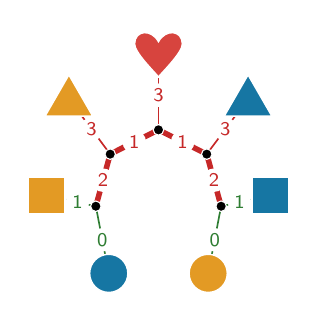
\begin{tikzpicture}[x=1.0cm,y=1.0cm,baseline=(current bounding box.center)]
\coordinate (v1) at (1.41868,-0.32381);
\coordinate (v2) at (1.13770,0.90728);
\coordinate (v3) at (-0.63137,-1.31106);
\coordinate (v4) at (-1.41868,-0.32381);
\coordinate (v5) at (-1.13770,0.90728);
\coordinate (v6) at (0.63137,-1.31106);
\coordinate (v7) at (0.00000,1.45517);
\coordinate (v8) at (0.79549,-0.45877);
\coordinate (v9) at (-0.79549,-0.45877);
\coordinate (v10) at (0.61308,0.20295);
\coordinate (v11) at (-0.61308,0.20295);
\coordinate (v12) at (-0.00000,0.51163);
\draw[g2tree internal,draw=g2Barren] (v8)--(v10);
\draw[g2tree internal,draw=g2Barren] (v9)--(v11);
\draw[g2tree internal,draw=g2Barren] (v10)--(v12);
\draw[g2tree internal,draw=g2Barren] (v11)--(v12);
\draw[g2tree pendant,draw=g2Prime] (v1)--(v8);
\draw[g2tree pendant,draw=g2Barren] (v2)--(v10);
\draw[g2tree pendant,draw=g2Prime] (v3)--(v9);
\draw[g2tree pendant,draw=g2Prime] (v4)--(v9);
\draw[g2tree pendant,draw=g2Barren] (v5)--(v11);
\draw[g2tree pendant,draw=g2Prime] (v6)--(v8);
\draw[g2tree pendant,draw=g2Barren] (v7)--(v12);
\node[g2tree weight,text=g2Barren,font={\sffamily\fontsize{7.5}{8}\selectfont}] at (0.70428,-0.12791) {2};
\node[g2tree weight,text=g2Barren,font={\sffamily\fontsize{7.5}{8}\selectfont}] at (-0.70428,-0.12791) {2};
\node[g2tree weight,text=g2Barren,font={\sffamily\fontsize{7.5}{8}\selectfont}] at (0.30654,0.35729) {1};
\node[g2tree weight,text=g2Barren,font={\sffamily\fontsize{7.5}{8}\selectfont}] at (-0.30654,0.35729) {1};
\node[g2tree weight,text=g2Prime,font={\sffamily\fontsize{7.5}{8}\selectfont}] at (1.02919,-0.40816) {1};
\node[g2tree weight,text=g2Barren,font={\sffamily\fontsize{7.5}{8}\selectfont}] at (0.84916,0.51990) {3};
\node[g2tree weight,text=g2Prime,font={\sffamily\fontsize{7.5}{8}\selectfont}] at (-0.71343,-0.88491) {0};
\node[g2tree weight,text=g2Prime,font={\sffamily\fontsize{7.5}{8}\selectfont}] at (-1.02919,-0.40816) {1};
\node[g2tree weight,text=g2Barren,font={\sffamily\fontsize{7.5}{8}\selectfont}] at (-0.84916,0.51990) {3};
\node[g2tree weight,text=g2Prime,font={\sffamily\fontsize{7.5}{8}\selectfont}] at (0.71343,-0.88491) {0};
\node[g2tree weight,text=g2Barren,font={\sffamily\fontsize{7.5}{8}\selectfont}] at (0.00000,0.95100) {3};
\node[g2tree vertex] at (v8) {};
\node[g2tree vertex] at (v9) {};
\node[g2tree vertex] at (v10) {};
\node[g2tree vertex] at (v11) {};
\node[g2tree vertex] at (v12) {};
\node[g2tree dark,rectangle,minimum size=4.657500000000001mm,font={\sffamily\fontsize{9}{9}\selectfont\bfseries}] at (v1) {};
\begin{scope}[shift={(v2)},scale=1.0125000000000002,transform shape]
\path[fill=g2TaxonBlue,draw=white,line width=.55pt,line join=round] (0mm,3.0mm)--(-3.0mm,-2.2mm)--(3.0mm,-2.2mm)--cycle;
\end{scope}
\node[g2tree dark,circle,minimum size=4.86mm,font={\sffamily\fontsize{9}{9}\selectfont\bfseries}] at (v3) {};
\node[g2tree light,rectangle,minimum size=4.657500000000001mm,font={\sffamily\fontsize{9}{9}\selectfont\bfseries}] at (v4) {};
\begin{scope}[shift={(v5)},scale=1.0125000000000002,transform shape]
\path[fill=g2TaxonYellow,draw=white,line width=.55pt,line join=round] (0mm,3.0mm)--(-3.0mm,-2.2mm)--(3.0mm,-2.2mm)--cycle;
\end{scope}
\node[g2tree light,circle,minimum size=4.86mm,font={\sffamily\fontsize{9}{9}\selectfont\bfseries}] at (v6) {};
\begin{scope}[shift={(v7)},scale=1.0125000000000002,transform shape]
\path[fill=g2HeartRed,draw=white,line width=.55pt]
  (0mm,-2.7mm)..controls(-.45mm,-2.1mm)and(-3.0mm,.35mm)..(-3.0mm,1.45mm)
  ..controls(-3.0mm,3.2mm)and(-.9mm,3.4mm)..(0mm,1.75mm)
  ..controls(.9mm,3.4mm)and(3.0mm,3.2mm)..(3.0mm,1.45mm)
  ..controls(3.0mm,.35mm)and(.45mm,-2.1mm)..(0mm,-2.7mm)--cycle;
\end{scope}
\end{tikzpicture}
\endgroup
\par}
\end{minipage}
 & 
\begin{minipage}[t]{\linewidth}
\noindent\textcolor{g2TreeRule}{\rule{\linewidth}{1pt}}\par
\noindent\textcolor[HTML]{000000}{\smash[b]{\textpdfrender{TextRenderingMode=FillStroke,LineWidth=.5pt}{\Large\bfseries\boldmath \oldstylenums{2}}{\large(6)}}}\hfill\textcolor{g2Prime}{\large4}\,\smash[b]{\tikz[baseline=0pt]\pic[scale=0.62] at (0,3.596mm) {g2apple};}\par
\vskip -1.2mm
{\centering
\begingroup
\definecolor{g2TaxonBlue}{HTML}{1676A3}
\definecolor{g2TaxonYellow}{HTML}{E39A24}
\definecolor{g2HeartRed}{HTML}{D7443E}
\tikzset{
  g2tree pendant/.style={draw=black,line width=.6pt,line cap=round},
  g2tree internal/.style={draw=black,line width=2pt,line cap=round},
  g2tree vertex/.style={circle,fill=black,draw=white,line width=.4pt,inner sep=0pt,minimum size=3.8pt},
  g2tree dark/.style={fill=g2TaxonBlue,draw=white,line width=.55pt,text=white,inner sep=0pt},
  g2tree light/.style={fill=g2TaxonYellow,draw=white,line width=.55pt,text=white,inner sep=0pt},
  g2tree weight/.style={circle,fill=white,draw=none,text=black,inner sep=.15pt,minimum size=8.5pt},
  g2tree aligned pendant/.style={fill=white,text=black,inner sep=.7pt,sloped,above=1pt,font={\sffamily\fontsize{7.5}{8}\selectfont}},
  g2tree aligned internal/.style={fill=white,text=black,inner sep=1pt,sloped,above=1pt,font={\sffamily\fontsize{7.5}{8}\selectfont\bfseries}},
}
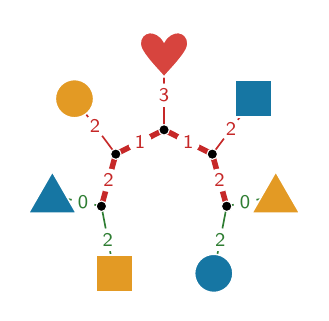
\begin{tikzpicture}[x=1.0cm,y=1.0cm,baseline=(current bounding box.center)]
\coordinate (v1) at (1.13770,0.90728);
\coordinate (v2) at (-1.41868,-0.32381);
\coordinate (v3) at (0.63137,-1.31106);
\coordinate (v4) at (-0.63137,-1.31106);
\coordinate (v5) at (1.41868,-0.32381);
\coordinate (v6) at (-1.13770,0.90728);
\coordinate (v7) at (0.00000,1.45517);
\coordinate (v8) at (-0.79549,-0.45877);
\coordinate (v9) at (0.79549,-0.45877);
\coordinate (v10) at (0.61308,0.20295);
\coordinate (v11) at (-0.61308,0.20295);
\coordinate (v12) at (-0.00000,0.51163);
\draw[g2tree internal,draw=g2Barren] (v8)--(v11);
\draw[g2tree internal,draw=g2Barren] (v9)--(v10);
\draw[g2tree internal,draw=g2Barren] (v10)--(v12);
\draw[g2tree internal,draw=g2Barren] (v11)--(v12);
\draw[g2tree pendant,draw=g2Barren] (v1)--(v10);
\draw[g2tree pendant,draw=g2Prime] (v2)--(v8);
\draw[g2tree pendant,draw=g2Prime] (v3)--(v9);
\draw[g2tree pendant,draw=g2Prime] (v4)--(v8);
\draw[g2tree pendant,draw=g2Prime] (v5)--(v9);
\draw[g2tree pendant,draw=g2Barren] (v6)--(v11);
\draw[g2tree pendant,draw=g2Barren] (v7)--(v12);
\node[g2tree weight,text=g2Barren,font={\sffamily\fontsize{7.5}{8}\selectfont}] at (-0.70428,-0.12791) {2};
\node[g2tree weight,text=g2Barren,font={\sffamily\fontsize{7.5}{8}\selectfont}] at (0.70428,-0.12791) {2};
\node[g2tree weight,text=g2Barren,font={\sffamily\fontsize{7.5}{8}\selectfont}] at (0.30654,0.35729) {1};
\node[g2tree weight,text=g2Barren,font={\sffamily\fontsize{7.5}{8}\selectfont}] at (-0.30654,0.35729) {1};
\node[g2tree weight,text=g2Barren,font={\sffamily\fontsize{7.5}{8}\selectfont}] at (0.84916,0.51990) {2};
\node[g2tree weight,text=g2Prime,font={\sffamily\fontsize{7.5}{8}\selectfont}] at (-1.02919,-0.40816) {0};
\node[g2tree weight,text=g2Prime,font={\sffamily\fontsize{7.5}{8}\selectfont}] at (0.71343,-0.88491) {2};
\node[g2tree weight,text=g2Prime,font={\sffamily\fontsize{7.5}{8}\selectfont}] at (-0.71343,-0.88491) {2};
\node[g2tree weight,text=g2Prime,font={\sffamily\fontsize{7.5}{8}\selectfont}] at (1.02919,-0.40816) {0};
\node[g2tree weight,text=g2Barren,font={\sffamily\fontsize{7.5}{8}\selectfont}] at (-0.87539,0.55512) {2};
\node[g2tree weight,text=g2Barren,font={\sffamily\fontsize{7.5}{8}\selectfont}] at (0.00000,0.95100) {3};
\node[g2tree vertex] at (v8) {};
\node[g2tree vertex] at (v9) {};
\node[g2tree vertex] at (v10) {};
\node[g2tree vertex] at (v11) {};
\node[g2tree vertex] at (v12) {};
\node[g2tree dark,rectangle,minimum size=4.657500000000001mm,font={\sffamily\fontsize{9}{9}\selectfont\bfseries}] at (v1) {};
\begin{scope}[shift={(v2)},scale=1.0125000000000002,transform shape]
\path[fill=g2TaxonBlue,draw=white,line width=.55pt,line join=round] (0mm,3.0mm)--(-3.0mm,-2.2mm)--(3.0mm,-2.2mm)--cycle;
\end{scope}
\node[g2tree dark,circle,minimum size=4.86mm,font={\sffamily\fontsize{9}{9}\selectfont\bfseries}] at (v3) {};
\node[g2tree light,rectangle,minimum size=4.657500000000001mm,font={\sffamily\fontsize{9}{9}\selectfont\bfseries}] at (v4) {};
\begin{scope}[shift={(v5)},scale=1.0125000000000002,transform shape]
\path[fill=g2TaxonYellow,draw=white,line width=.55pt,line join=round] (0mm,3.0mm)--(-3.0mm,-2.2mm)--(3.0mm,-2.2mm)--cycle;
\end{scope}
\node[g2tree light,circle,minimum size=4.86mm,font={\sffamily\fontsize{9}{9}\selectfont\bfseries}] at (v6) {};
\begin{scope}[shift={(v7)},scale=1.0125000000000002,transform shape]
\path[fill=g2HeartRed,draw=white,line width=.55pt]
  (0mm,-2.7mm)..controls(-.45mm,-2.1mm)and(-3.0mm,.35mm)..(-3.0mm,1.45mm)
  ..controls(-3.0mm,3.2mm)and(-.9mm,3.4mm)..(0mm,1.75mm)
  ..controls(.9mm,3.4mm)and(3.0mm,3.2mm)..(3.0mm,1.45mm)
  ..controls(3.0mm,.35mm)and(.45mm,-2.1mm)..(0mm,-2.7mm)--cycle;
\end{scope}
\end{tikzpicture}
\endgroup
\par}
\end{minipage}
 & 
\begin{minipage}[t]{\linewidth}
\noindent\textcolor{g2TreeRule}{\rule{\linewidth}{1pt}}\par
\noindent\textcolor[HTML]{000000}{\smash[b]{\textpdfrender{TextRenderingMode=FillStroke,LineWidth=.5pt}{\Large\bfseries\boldmath \oldstylenums{3}}{\large(12)}}}\hfill\textcolor{g2Prime}{\large6}\,\smash[b]{\tikz[baseline=0pt]\pic[scale=0.62] at (0,3.596mm) {g2apple};}\par
\vskip -1.2mm
{\centering
\begingroup
\definecolor{g2TaxonBlue}{HTML}{1676A3}
\definecolor{g2TaxonYellow}{HTML}{E39A24}
\definecolor{g2HeartRed}{HTML}{D7443E}
\tikzset{
  g2tree pendant/.style={draw=black,line width=.6pt,line cap=round},
  g2tree internal/.style={draw=black,line width=2pt,line cap=round},
  g2tree vertex/.style={circle,fill=black,draw=white,line width=.4pt,inner sep=0pt,minimum size=3.8pt},
  g2tree dark/.style={fill=g2TaxonBlue,draw=white,line width=.55pt,text=white,inner sep=0pt},
  g2tree light/.style={fill=g2TaxonYellow,draw=white,line width=.55pt,text=white,inner sep=0pt},
  g2tree weight/.style={circle,fill=white,draw=none,text=black,inner sep=.15pt,minimum size=8.5pt},
  g2tree aligned pendant/.style={fill=white,text=black,inner sep=.7pt,sloped,above=1pt,font={\sffamily\fontsize{7.5}{8}\selectfont}},
  g2tree aligned internal/.style={fill=white,text=black,inner sep=1pt,sloped,above=1pt,font={\sffamily\fontsize{7.5}{8}\selectfont\bfseries}},
}
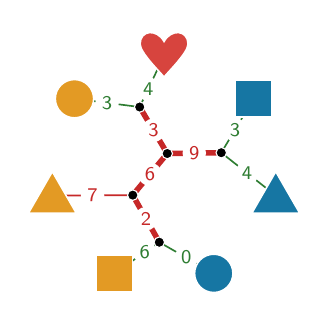
\begin{tikzpicture}[x=1.0cm,y=1.0cm,baseline=(current bounding box.center)]
\coordinate (v1) at (1.13770,0.90728);
\coordinate (v2) at (1.41868,-0.32381);
\coordinate (v3) at (0.63137,-1.31106);
\coordinate (v4) at (-0.63137,-1.31106);
\coordinate (v5) at (-1.41868,-0.32381);
\coordinate (v6) at (-1.13770,0.90728);
\coordinate (v7) at (0.00000,1.45517);
\coordinate (v8) at (0.72681,0.22115);
\coordinate (v9) at (-0.30939,0.80136);
\coordinate (v10) at (0.04049,0.21082);
\coordinate (v11) at (-0.06043,-0.91564);
\coordinate (v12) at (-0.39748,-0.31769);
\draw[g2tree internal,draw=g2Barren] (v8)--(v10);
\draw[g2tree internal,draw=g2Barren] (v9)--(v10);
\draw[g2tree internal,draw=g2Barren] (v10)--(v12);
\draw[g2tree internal,draw=g2Barren] (v11)--(v12);
\draw[g2tree pendant,draw=g2Prime] (v1)--(v8);
\draw[g2tree pendant,draw=g2Prime] (v2)--(v8);
\draw[g2tree pendant,draw=g2Prime] (v3)--(v11);
\draw[g2tree pendant,draw=g2Prime] (v4)--(v11);
\draw[g2tree pendant,draw=g2Barren] (v5)--(v12);
\draw[g2tree pendant,draw=g2Prime] (v6)--(v9);
\draw[g2tree pendant,draw=g2Prime] (v7)--(v9);
\node[g2tree weight,text=g2Barren,font={\sffamily\fontsize{7.5}{8}\selectfont}] at (0.38365,0.21599) {9};
\node[g2tree weight,text=g2Barren,font={\sffamily\fontsize{7.5}{8}\selectfont}] at (-0.13445,0.50609) {3};
\node[g2tree weight,text=g2Barren,font={\sffamily\fontsize{7.5}{8}\selectfont}] at (-0.17850,-0.05343) {6};
\node[g2tree weight,text=g2Barren,font={\sffamily\fontsize{7.5}{8}\selectfont}] at (-0.22895,-0.61666) {2};
\node[g2tree weight,text=g2Prime,font={\sffamily\fontsize{7.5}{8}\selectfont}] at (0.90144,0.51275) {3};
\node[g2tree weight,text=g2Prime,font={\sffamily\fontsize{7.5}{8}\selectfont}] at (1.05444,-0.03691) {4};
\node[g2tree weight,text=g2Prime,font={\sffamily\fontsize{7.5}{8}\selectfont}] at (0.28157,-1.11112) {0};
\node[g2tree weight,text=g2Prime,font={\sffamily\fontsize{7.5}{8}\selectfont}] at (-0.24599,-1.04415) {6};
\node[g2tree weight,text=g2Barren,font={\sffamily\fontsize{7.5}{8}\selectfont}] at (-0.90808,-0.32075) {7};
\node[g2tree weight,text=g2Prime,font={\sffamily\fontsize{7.5}{8}\selectfont}] at (-0.72354,0.85432) {3};
\node[g2tree weight,text=g2Prime,font={\sffamily\fontsize{7.5}{8}\selectfont}] at (-0.20110,1.03019) {4};
\node[g2tree vertex] at (v8) {};
\node[g2tree vertex] at (v9) {};
\node[g2tree vertex] at (v10) {};
\node[g2tree vertex] at (v11) {};
\node[g2tree vertex] at (v12) {};
\node[g2tree dark,rectangle,minimum size=4.657500000000001mm,font={\sffamily\fontsize{9}{9}\selectfont\bfseries}] at (v1) {};
\begin{scope}[shift={(v2)},scale=1.0125000000000002,transform shape]
\path[fill=g2TaxonBlue,draw=white,line width=.55pt,line join=round] (0mm,3.0mm)--(-3.0mm,-2.2mm)--(3.0mm,-2.2mm)--cycle;
\end{scope}
\node[g2tree dark,circle,minimum size=4.86mm,font={\sffamily\fontsize{9}{9}\selectfont\bfseries}] at (v3) {};
\node[g2tree light,rectangle,minimum size=4.657500000000001mm,font={\sffamily\fontsize{9}{9}\selectfont\bfseries}] at (v4) {};
\begin{scope}[shift={(v5)},scale=1.0125000000000002,transform shape]
\path[fill=g2TaxonYellow,draw=white,line width=.55pt,line join=round] (0mm,3.0mm)--(-3.0mm,-2.2mm)--(3.0mm,-2.2mm)--cycle;
\end{scope}
\node[g2tree light,circle,minimum size=4.86mm,font={\sffamily\fontsize{9}{9}\selectfont\bfseries}] at (v6) {};
\begin{scope}[shift={(v7)},scale=1.0125000000000002,transform shape]
\path[fill=g2HeartRed,draw=white,line width=.55pt]
  (0mm,-2.7mm)..controls(-.45mm,-2.1mm)and(-3.0mm,.35mm)..(-3.0mm,1.45mm)
  ..controls(-3.0mm,3.2mm)and(-.9mm,3.4mm)..(0mm,1.75mm)
  ..controls(.9mm,3.4mm)and(3.0mm,3.2mm)..(3.0mm,1.45mm)
  ..controls(3.0mm,.35mm)and(.45mm,-2.1mm)..(0mm,-2.7mm)--cycle;
\end{scope}
\end{tikzpicture}
\endgroup
\par}
\end{minipage}
 & 
\begin{minipage}[t]{\linewidth}
\noindent\textcolor{g2TreeRule}{\rule{\linewidth}{1pt}}\par
\noindent\textcolor[HTML]{000000}{\smash[b]{\textpdfrender{TextRenderingMode=FillStroke,LineWidth=.5pt}{\Large\bfseries\boldmath \oldstylenums{4}}{\large(12)}}}\hfill\textcolor{g2Prime}{\large6}\,\smash[b]{\tikz[baseline=0pt]\pic[scale=0.62] at (0,3.596mm) {g2apple};}\par
\vskip -1.2mm
{\centering
\begingroup
\definecolor{g2TaxonBlue}{HTML}{1676A3}
\definecolor{g2TaxonYellow}{HTML}{E39A24}
\definecolor{g2HeartRed}{HTML}{D7443E}
\tikzset{
  g2tree pendant/.style={draw=black,line width=.6pt,line cap=round},
  g2tree internal/.style={draw=black,line width=2pt,line cap=round},
  g2tree vertex/.style={circle,fill=black,draw=white,line width=.4pt,inner sep=0pt,minimum size=3.8pt},
  g2tree dark/.style={fill=g2TaxonBlue,draw=white,line width=.55pt,text=white,inner sep=0pt},
  g2tree light/.style={fill=g2TaxonYellow,draw=white,line width=.55pt,text=white,inner sep=0pt},
  g2tree weight/.style={circle,fill=white,draw=none,text=black,inner sep=.15pt,minimum size=8.5pt},
  g2tree aligned pendant/.style={fill=white,text=black,inner sep=.7pt,sloped,above=1pt,font={\sffamily\fontsize{7.5}{8}\selectfont}},
  g2tree aligned internal/.style={fill=white,text=black,inner sep=1pt,sloped,above=1pt,font={\sffamily\fontsize{7.5}{8}\selectfont\bfseries}},
}
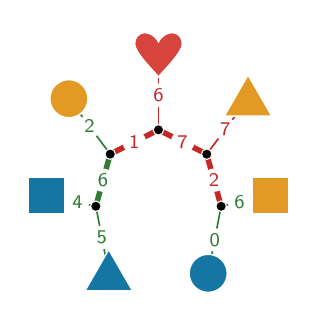
\begin{tikzpicture}[x=1.0cm,y=1.0cm,baseline=(current bounding box.center)]
\coordinate (v1) at (-1.41868,-0.32381);
\coordinate (v2) at (-0.63137,-1.31106);
\coordinate (v3) at (0.63137,-1.31106);
\coordinate (v4) at (1.41868,-0.32381);
\coordinate (v5) at (1.13770,0.90728);
\coordinate (v6) at (-1.13770,0.90728);
\coordinate (v7) at (0.00000,1.45517);
\coordinate (v8) at (-0.79549,-0.45877);
\coordinate (v9) at (0.79549,-0.45877);
\coordinate (v10) at (0.61308,0.20295);
\coordinate (v11) at (-0.61308,0.20295);
\coordinate (v12) at (-0.00000,0.51163);
\draw[g2tree internal,draw=g2Prime] (v8)--(v11);
\draw[g2tree internal,draw=g2Barren] (v9)--(v10);
\draw[g2tree internal,draw=g2Barren] (v10)--(v12);
\draw[g2tree internal,draw=g2Barren] (v11)--(v12);
\draw[g2tree pendant,draw=g2Prime] (v1)--(v8);
\draw[g2tree pendant,draw=g2Prime] (v2)--(v8);
\draw[g2tree pendant,draw=g2Prime] (v3)--(v9);
\draw[g2tree pendant,draw=g2Prime] (v4)--(v9);
\draw[g2tree pendant,draw=g2Barren] (v5)--(v10);
\draw[g2tree pendant,draw=g2Prime] (v6)--(v11);
\draw[g2tree pendant,draw=g2Barren] (v7)--(v12);
\node[g2tree weight,text=g2Prime,font={\sffamily\fontsize{7.5}{8}\selectfont}] at (-0.70428,-0.12791) {6};
\node[g2tree weight,text=g2Barren,font={\sffamily\fontsize{7.5}{8}\selectfont}] at (0.70428,-0.12791) {2};
\node[g2tree weight,text=g2Barren,font={\sffamily\fontsize{7.5}{8}\selectfont}] at (0.30654,0.35729) {7};
\node[g2tree weight,text=g2Barren,font={\sffamily\fontsize{7.5}{8}\selectfont}] at (-0.30654,0.35729) {1};
\node[g2tree weight,text=g2Prime,font={\sffamily\fontsize{7.5}{8}\selectfont}] at (-1.02919,-0.40816) {4};
\node[g2tree weight,text=g2Prime,font={\sffamily\fontsize{7.5}{8}\selectfont}] at (-0.71905,-0.85576) {5};
\node[g2tree weight,text=g2Prime,font={\sffamily\fontsize{7.5}{8}\selectfont}] at (0.71343,-0.88491) {0};
\node[g2tree weight,text=g2Prime,font={\sffamily\fontsize{7.5}{8}\selectfont}] at (1.02919,-0.40816) {6};
\node[g2tree weight,text=g2Barren,font={\sffamily\fontsize{7.5}{8}\selectfont}] at (0.84916,0.51990) {7};
\node[g2tree weight,text=g2Prime,font={\sffamily\fontsize{7.5}{8}\selectfont}] at (-0.87539,0.55512) {2};
\node[g2tree weight,text=g2Barren,font={\sffamily\fontsize{7.5}{8}\selectfont}] at (0.00000,0.95100) {6};
\node[g2tree vertex] at (v8) {};
\node[g2tree vertex] at (v9) {};
\node[g2tree vertex] at (v10) {};
\node[g2tree vertex] at (v11) {};
\node[g2tree vertex] at (v12) {};
\node[g2tree dark,rectangle,minimum size=4.657500000000001mm,font={\sffamily\fontsize{9}{9}\selectfont\bfseries}] at (v1) {};
\begin{scope}[shift={(v2)},scale=1.0125000000000002,transform shape]
\path[fill=g2TaxonBlue,draw=white,line width=.55pt,line join=round] (0mm,3.0mm)--(-3.0mm,-2.2mm)--(3.0mm,-2.2mm)--cycle;
\end{scope}
\node[g2tree dark,circle,minimum size=4.86mm,font={\sffamily\fontsize{9}{9}\selectfont\bfseries}] at (v3) {};
\node[g2tree light,rectangle,minimum size=4.657500000000001mm,font={\sffamily\fontsize{9}{9}\selectfont\bfseries}] at (v4) {};
\begin{scope}[shift={(v5)},scale=1.0125000000000002,transform shape]
\path[fill=g2TaxonYellow,draw=white,line width=.55pt,line join=round] (0mm,3.0mm)--(-3.0mm,-2.2mm)--(3.0mm,-2.2mm)--cycle;
\end{scope}
\node[g2tree light,circle,minimum size=4.86mm,font={\sffamily\fontsize{9}{9}\selectfont\bfseries}] at (v6) {};
\begin{scope}[shift={(v7)},scale=1.0125000000000002,transform shape]
\path[fill=g2HeartRed,draw=white,line width=.55pt]
  (0mm,-2.7mm)..controls(-.45mm,-2.1mm)and(-3.0mm,.35mm)..(-3.0mm,1.45mm)
  ..controls(-3.0mm,3.2mm)and(-.9mm,3.4mm)..(0mm,1.75mm)
  ..controls(.9mm,3.4mm)and(3.0mm,3.2mm)..(3.0mm,1.45mm)
  ..controls(3.0mm,.35mm)and(.45mm,-2.1mm)..(0mm,-2.7mm)--cycle;
\end{scope}
\end{tikzpicture}
\endgroup
\par}
\end{minipage}
\\\noalign{\vskip 0.485cm}
\begin{minipage}[t]{\linewidth}
\noindent\textcolor{g2TreeRule}{\rule{\linewidth}{1pt}}\par
\noindent\textcolor[HTML]{000000}{\smash[b]{\textpdfrender{TextRenderingMode=FillStroke,LineWidth=.5pt}{\Large\bfseries\boldmath \oldstylenums{5}}{\large(6)}}}\hfill\textcolor{g2Prime}{\large8}\,\smash[b]{\tikz[baseline=0pt]\pic[scale=0.62] at (0,3.596mm) {g2apple};}\par
\vskip -1.2mm
{\centering
\begingroup
\definecolor{g2TaxonBlue}{HTML}{1676A3}
\definecolor{g2TaxonYellow}{HTML}{E39A24}
\definecolor{g2HeartRed}{HTML}{D7443E}
\tikzset{
  g2tree pendant/.style={draw=black,line width=.6pt,line cap=round},
  g2tree internal/.style={draw=black,line width=2pt,line cap=round},
  g2tree vertex/.style={circle,fill=black,draw=white,line width=.4pt,inner sep=0pt,minimum size=3.8pt},
  g2tree dark/.style={fill=g2TaxonBlue,draw=white,line width=.55pt,text=white,inner sep=0pt},
  g2tree light/.style={fill=g2TaxonYellow,draw=white,line width=.55pt,text=white,inner sep=0pt},
  g2tree weight/.style={circle,fill=white,draw=none,text=black,inner sep=.15pt,minimum size=8.5pt},
  g2tree aligned pendant/.style={fill=white,text=black,inner sep=.7pt,sloped,above=1pt,font={\sffamily\fontsize{7.5}{8}\selectfont}},
  g2tree aligned internal/.style={fill=white,text=black,inner sep=1pt,sloped,above=1pt,font={\sffamily\fontsize{7.5}{8}\selectfont\bfseries}},
}
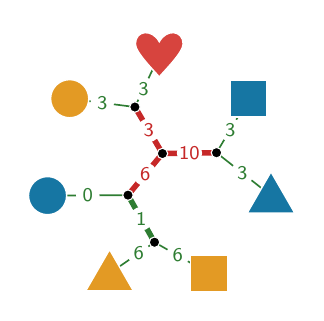
\begin{tikzpicture}[x=1.0cm,y=1.0cm,baseline=(current bounding box.center)]
\coordinate (v1) at (1.13770,0.90728);
\coordinate (v2) at (1.41868,-0.32381);
\coordinate (v3) at (-1.41868,-0.32381);
\coordinate (v4) at (0.63137,-1.31106);
\coordinate (v5) at (-0.63137,-1.31106);
\coordinate (v6) at (-1.13770,0.90728);
\coordinate (v7) at (0.00000,1.45517);
\coordinate (v8) at (0.72681,0.22115);
\coordinate (v9) at (-0.30939,0.80136);
\coordinate (v10) at (0.04049,0.21082);
\coordinate (v11) at (-0.39748,-0.31769);
\coordinate (v12) at (-0.06043,-0.91564);
\draw[g2tree internal,draw=g2Barren] (v8)--(v10);
\draw[g2tree internal,draw=g2Barren] (v9)--(v10);
\draw[g2tree internal,draw=g2Barren] (v10)--(v11);
\draw[g2tree internal,draw=g2Prime] (v11)--(v12);
\draw[g2tree pendant,draw=g2Prime] (v1)--(v8);
\draw[g2tree pendant,draw=g2Prime] (v2)--(v8);
\draw[g2tree pendant,draw=g2Prime] (v3)--(v11);
\draw[g2tree pendant,draw=g2Prime] (v4)--(v12);
\draw[g2tree pendant,draw=g2Prime] (v5)--(v12);
\draw[g2tree pendant,draw=g2Prime] (v6)--(v9);
\draw[g2tree pendant,draw=g2Prime] (v7)--(v9);
\node[g2tree weight,text=g2Barren,font={\sffamily\fontsize{7.5}{8}\selectfont}] at (0.38365,0.21599) {10};
\node[g2tree weight,text=g2Barren,font={\sffamily\fontsize{7.5}{8}\selectfont}] at (-0.13445,0.50609) {3};
\node[g2tree weight,text=g2Barren,font={\sffamily\fontsize{7.5}{8}\selectfont}] at (-0.17850,-0.05343) {6};
\node[g2tree weight,text=g2Prime,font={\sffamily\fontsize{7.5}{8}\selectfont}] at (-0.22895,-0.61666) {1};
\node[g2tree weight,text=g2Prime,font={\sffamily\fontsize{7.5}{8}\selectfont}] at (0.90144,0.51275) {3};
\node[g2tree weight,text=g2Prime,font={\sffamily\fontsize{7.5}{8}\selectfont}] at (1.05444,-0.03691) {3};
\node[g2tree weight,text=g2Prime,font={\sffamily\fontsize{7.5}{8}\selectfont}] at (-0.90808,-0.32075) {0};
\node[g2tree weight,text=g2Prime,font={\sffamily\fontsize{7.5}{8}\selectfont}] at (0.23359,-1.08369) {6};
\node[g2tree weight,text=g2Prime,font={\sffamily\fontsize{7.5}{8}\selectfont}] at (-0.26026,-1.05404) {6};
\node[g2tree weight,text=g2Prime,font={\sffamily\fontsize{7.5}{8}\selectfont}] at (-0.72354,0.85432) {3};
\node[g2tree weight,text=g2Prime,font={\sffamily\fontsize{7.5}{8}\selectfont}] at (-0.20110,1.03019) {3};
\node[g2tree vertex] at (v8) {};
\node[g2tree vertex] at (v9) {};
\node[g2tree vertex] at (v10) {};
\node[g2tree vertex] at (v11) {};
\node[g2tree vertex] at (v12) {};
\node[g2tree dark,rectangle,minimum size=4.657500000000001mm,font={\sffamily\fontsize{9}{9}\selectfont\bfseries}] at (v1) {};
\begin{scope}[shift={(v2)},scale=1.0125000000000002,transform shape]
\path[fill=g2TaxonBlue,draw=white,line width=.55pt,line join=round] (0mm,3.0mm)--(-3.0mm,-2.2mm)--(3.0mm,-2.2mm)--cycle;
\end{scope}
\node[g2tree dark,circle,minimum size=4.86mm,font={\sffamily\fontsize{9}{9}\selectfont\bfseries}] at (v3) {};
\node[g2tree light,rectangle,minimum size=4.657500000000001mm,font={\sffamily\fontsize{9}{9}\selectfont\bfseries}] at (v4) {};
\begin{scope}[shift={(v5)},scale=1.0125000000000002,transform shape]
\path[fill=g2TaxonYellow,draw=white,line width=.55pt,line join=round] (0mm,3.0mm)--(-3.0mm,-2.2mm)--(3.0mm,-2.2mm)--cycle;
\end{scope}
\node[g2tree light,circle,minimum size=4.86mm,font={\sffamily\fontsize{9}{9}\selectfont\bfseries}] at (v6) {};
\begin{scope}[shift={(v7)},scale=1.0125000000000002,transform shape]
\path[fill=g2HeartRed,draw=white,line width=.55pt]
  (0mm,-2.7mm)..controls(-.45mm,-2.1mm)and(-3.0mm,.35mm)..(-3.0mm,1.45mm)
  ..controls(-3.0mm,3.2mm)and(-.9mm,3.4mm)..(0mm,1.75mm)
  ..controls(.9mm,3.4mm)and(3.0mm,3.2mm)..(3.0mm,1.45mm)
  ..controls(3.0mm,.35mm)and(.45mm,-2.1mm)..(0mm,-2.7mm)--cycle;
\end{scope}
\end{tikzpicture}
\endgroup
\par}
\end{minipage}
 & 
\begin{minipage}[t]{\linewidth}
\noindent\textcolor{g2TreeRule}{\rule{\linewidth}{1pt}}\par
\noindent\textcolor[HTML]{000000}{\smash[b]{\textpdfrender{TextRenderingMode=FillStroke,LineWidth=.5pt}{\Large\bfseries\boldmath \oldstylenums{6}}{\large(3)}}}\hfill\textcolor{g2Prime}{\large6}\,\smash[b]{\tikz[baseline=0pt]\pic[scale=0.62] at (0,3.596mm) {g2apple};}\par
\vskip -1.2mm
{\centering
\begingroup
\definecolor{g2TaxonBlue}{HTML}{1676A3}
\definecolor{g2TaxonYellow}{HTML}{E39A24}
\definecolor{g2HeartRed}{HTML}{D7443E}
\tikzset{
  g2tree pendant/.style={draw=black,line width=.6pt,line cap=round},
  g2tree internal/.style={draw=black,line width=2pt,line cap=round},
  g2tree vertex/.style={circle,fill=black,draw=white,line width=.4pt,inner sep=0pt,minimum size=3.8pt},
  g2tree dark/.style={fill=g2TaxonBlue,draw=white,line width=.55pt,text=white,inner sep=0pt},
  g2tree light/.style={fill=g2TaxonYellow,draw=white,line width=.55pt,text=white,inner sep=0pt},
  g2tree weight/.style={circle,fill=white,draw=none,text=black,inner sep=.15pt,minimum size=8.5pt},
  g2tree aligned pendant/.style={fill=white,text=black,inner sep=.7pt,sloped,above=1pt,font={\sffamily\fontsize{7.5}{8}\selectfont}},
  g2tree aligned internal/.style={fill=white,text=black,inner sep=1pt,sloped,above=1pt,font={\sffamily\fontsize{7.5}{8}\selectfont\bfseries}},
}
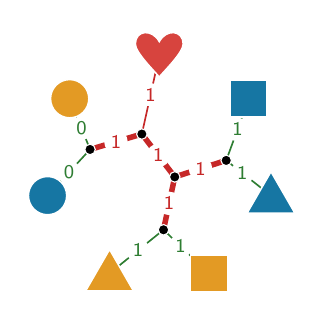
\begin{tikzpicture}[x=1.0cm,y=1.0cm,baseline=(current bounding box.center)]
\coordinate (v1) at (1.13770,0.90728);
\coordinate (v2) at (1.41868,-0.32381);
\coordinate (v3) at (-1.41868,-0.32381);
\coordinate (v4) at (0.63137,-1.31106);
\coordinate (v5) at (-0.63137,-1.31106);
\coordinate (v6) at (-1.13770,0.90728);
\coordinate (v7) at (0.00000,1.45517);
\coordinate (v8) at (-0.87924,0.26266);
\coordinate (v9) at (0.85011,0.12332);
\coordinate (v10) at (0.05387,-0.75780);
\coordinate (v11) at (-0.22128,0.45821);
\coordinate (v12) at (0.19653,-0.08639);
\draw[g2tree internal,draw=g2Barren] (v8)--(v11);
\draw[g2tree internal,draw=g2Barren] (v9)--(v12);
\draw[g2tree internal,draw=g2Barren] (v10)--(v12);
\draw[g2tree internal,draw=g2Barren] (v11)--(v12);
\draw[g2tree pendant,draw=g2Prime] (v1)--(v9);
\draw[g2tree pendant,draw=g2Prime] (v2)--(v9);
\draw[g2tree pendant,draw=g2Prime] (v3)--(v8);
\draw[g2tree pendant,draw=g2Prime] (v4)--(v10);
\draw[g2tree pendant,draw=g2Prime] (v5)--(v10);
\draw[g2tree pendant,draw=g2Prime] (v6)--(v8);
\draw[g2tree pendant,draw=g2Barren] (v7)--(v11);
\node[g2tree weight,text=g2Barren,font={\sffamily\fontsize{7.5}{8}\selectfont}] at (-0.55026,0.36043) {1};
\node[g2tree weight,text=g2Barren,font={\sffamily\fontsize{7.5}{8}\selectfont}] at (0.52332,0.01846) {1};
\node[g2tree weight,text=g2Barren,font={\sffamily\fontsize{7.5}{8}\selectfont}] at (0.12520,-0.42209) {1};
\node[g2tree weight,text=g2Barren,font={\sffamily\fontsize{7.5}{8}\selectfont}] at (-0.01237,0.18591) {1};
\node[g2tree weight,text=g2Prime,font={\sffamily\fontsize{7.5}{8}\selectfont}] at (0.99390,0.51530) {1};
\node[g2tree weight,text=g2Prime,font={\sffamily\fontsize{7.5}{8}\selectfont}] at (1.05422,-0.03719) {1};
\node[g2tree weight,text=g2Prime,font={\sffamily\fontsize{7.5}{8}\selectfont}] at (-1.14592,-0.02726) {0};
\node[g2tree weight,text=g2Prime,font={\sffamily\fontsize{7.5}{8}\selectfont}] at (0.27044,-0.96527) {1};
\node[g2tree weight,text=g2Prime,font={\sffamily\fontsize{7.5}{8}\selectfont}] at (-0.27062,-1.01979) {1};
\node[g2tree weight,text=g2Prime,font={\sffamily\fontsize{7.5}{8}\selectfont}] at (-0.98775,0.53331) {0};
\node[g2tree weight,text=g2Barren,font={\sffamily\fontsize{7.5}{8}\selectfont}] at (-0.11064,0.95669) {1};
\node[g2tree vertex] at (v8) {};
\node[g2tree vertex] at (v9) {};
\node[g2tree vertex] at (v10) {};
\node[g2tree vertex] at (v11) {};
\node[g2tree vertex] at (v12) {};
\node[g2tree dark,rectangle,minimum size=4.657500000000001mm,font={\sffamily\fontsize{9}{9}\selectfont\bfseries}] at (v1) {};
\begin{scope}[shift={(v2)},scale=1.0125000000000002,transform shape]
\path[fill=g2TaxonBlue,draw=white,line width=.55pt,line join=round] (0mm,3.0mm)--(-3.0mm,-2.2mm)--(3.0mm,-2.2mm)--cycle;
\end{scope}
\node[g2tree dark,circle,minimum size=4.86mm,font={\sffamily\fontsize{9}{9}\selectfont\bfseries}] at (v3) {};
\node[g2tree light,rectangle,minimum size=4.657500000000001mm,font={\sffamily\fontsize{9}{9}\selectfont\bfseries}] at (v4) {};
\begin{scope}[shift={(v5)},scale=1.0125000000000002,transform shape]
\path[fill=g2TaxonYellow,draw=white,line width=.55pt,line join=round] (0mm,3.0mm)--(-3.0mm,-2.2mm)--(3.0mm,-2.2mm)--cycle;
\end{scope}
\node[g2tree light,circle,minimum size=4.86mm,font={\sffamily\fontsize{9}{9}\selectfont\bfseries}] at (v6) {};
\begin{scope}[shift={(v7)},scale=1.0125000000000002,transform shape]
\path[fill=g2HeartRed,draw=white,line width=.55pt]
  (0mm,-2.7mm)..controls(-.45mm,-2.1mm)and(-3.0mm,.35mm)..(-3.0mm,1.45mm)
  ..controls(-3.0mm,3.2mm)and(-.9mm,3.4mm)..(0mm,1.75mm)
  ..controls(.9mm,3.4mm)and(3.0mm,3.2mm)..(3.0mm,1.45mm)
  ..controls(3.0mm,.35mm)and(.45mm,-2.1mm)..(0mm,-2.7mm)--cycle;
\end{scope}
\end{tikzpicture}
\endgroup
\par}
\end{minipage}
 & 
\begin{minipage}[t]{\linewidth}
\noindent\textcolor{g2TreeRule}{\rule{\linewidth}{1pt}}\par
\noindent\textcolor[HTML]{000000}{\smash[b]{\textpdfrender{TextRenderingMode=FillStroke,LineWidth=.5pt}{\Large\bfseries\boldmath \oldstylenums{7}}{\large(3)}}}\hfill\textcolor{g2Prime}{\large11}\,\smash[b]{\tikz[baseline=0pt]\pic[scale=0.62] at (0,3.596mm) {g2apple};}\par
\vskip -1.2mm
{\centering
\begingroup
\definecolor{g2TaxonBlue}{HTML}{1676A3}
\definecolor{g2TaxonYellow}{HTML}{E39A24}
\definecolor{g2HeartRed}{HTML}{D7443E}
\tikzset{
  g2tree pendant/.style={draw=black,line width=.6pt,line cap=round},
  g2tree internal/.style={draw=black,line width=2pt,line cap=round},
  g2tree vertex/.style={circle,fill=black,draw=white,line width=.4pt,inner sep=0pt,minimum size=3.8pt},
  g2tree dark/.style={fill=g2TaxonBlue,draw=white,line width=.55pt,text=white,inner sep=0pt},
  g2tree light/.style={fill=g2TaxonYellow,draw=white,line width=.55pt,text=white,inner sep=0pt},
  g2tree weight/.style={circle,fill=white,draw=none,text=black,inner sep=.15pt,minimum size=8.5pt},
  g2tree aligned pendant/.style={fill=white,text=black,inner sep=.7pt,sloped,above=1pt,font={\sffamily\fontsize{7.5}{8}\selectfont}},
  g2tree aligned internal/.style={fill=white,text=black,inner sep=1pt,sloped,above=1pt,font={\sffamily\fontsize{7.5}{8}\selectfont\bfseries}},
}
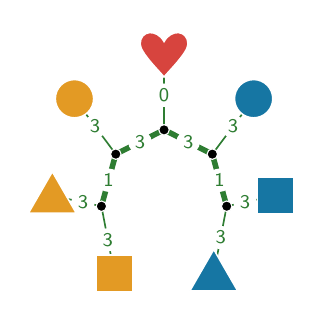
\begin{tikzpicture}[x=1.0cm,y=1.0cm,baseline=(current bounding box.center)]
\coordinate (v1) at (1.41868,-0.32381);
\coordinate (v2) at (0.63137,-1.31106);
\coordinate (v3) at (1.13770,0.90728);
\coordinate (v4) at (-0.63137,-1.31106);
\coordinate (v5) at (-1.41868,-0.32381);
\coordinate (v6) at (-1.13770,0.90728);
\coordinate (v7) at (0.00000,1.45517);
\coordinate (v8) at (0.79549,-0.45877);
\coordinate (v9) at (0.61308,0.20295);
\coordinate (v10) at (-0.00000,0.51163);
\coordinate (v11) at (-0.79549,-0.45877);
\coordinate (v12) at (-0.61308,0.20295);
\draw[g2tree internal,draw=g2Prime] (v8)--(v9);
\draw[g2tree internal,draw=g2Prime] (v9)--(v10);
\draw[g2tree internal,draw=g2Prime] (v10)--(v12);
\draw[g2tree internal,draw=g2Prime] (v11)--(v12);
\draw[g2tree pendant,draw=g2Prime] (v1)--(v8);
\draw[g2tree pendant,draw=g2Prime] (v2)--(v8);
\draw[g2tree pendant,draw=g2Prime] (v3)--(v9);
\draw[g2tree pendant,draw=g2Prime] (v4)--(v11);
\draw[g2tree pendant,draw=g2Prime] (v5)--(v11);
\draw[g2tree pendant,draw=g2Prime] (v6)--(v12);
\draw[g2tree pendant,draw=g2Prime] (v7)--(v10);
\node[g2tree weight,text=g2Prime,font={\sffamily\fontsize{7.5}{8}\selectfont}] at (0.70428,-0.12791) {1};
\node[g2tree weight,text=g2Prime,font={\sffamily\fontsize{7.5}{8}\selectfont}] at (0.30654,0.35729) {3};
\node[g2tree weight,text=g2Prime,font={\sffamily\fontsize{7.5}{8}\selectfont}] at (-0.30654,0.35729) {3};
\node[g2tree weight,text=g2Prime,font={\sffamily\fontsize{7.5}{8}\selectfont}] at (-0.70428,-0.12791) {1};
\node[g2tree weight,text=g2Prime,font={\sffamily\fontsize{7.5}{8}\selectfont}] at (1.02919,-0.40816) {3};
\node[g2tree weight,text=g2Prime,font={\sffamily\fontsize{7.5}{8}\selectfont}] at (0.71905,-0.85576) {3};
\node[g2tree weight,text=g2Prime,font={\sffamily\fontsize{7.5}{8}\selectfont}] at (0.87539,0.55512) {3};
\node[g2tree weight,text=g2Prime,font={\sffamily\fontsize{7.5}{8}\selectfont}] at (-0.71343,-0.88491) {3};
\node[g2tree weight,text=g2Prime,font={\sffamily\fontsize{7.5}{8}\selectfont}] at (-1.02919,-0.40816) {3};
\node[g2tree weight,text=g2Prime,font={\sffamily\fontsize{7.5}{8}\selectfont}] at (-0.87539,0.55512) {3};
\node[g2tree weight,text=g2Prime,font={\sffamily\fontsize{7.5}{8}\selectfont}] at (0.00000,0.95100) {0};
\node[g2tree vertex] at (v8) {};
\node[g2tree vertex] at (v9) {};
\node[g2tree vertex] at (v10) {};
\node[g2tree vertex] at (v11) {};
\node[g2tree vertex] at (v12) {};
\node[g2tree dark,rectangle,minimum size=4.657500000000001mm,font={\sffamily\fontsize{9}{9}\selectfont\bfseries}] at (v1) {};
\begin{scope}[shift={(v2)},scale=1.0125000000000002,transform shape]
\path[fill=g2TaxonBlue,draw=white,line width=.55pt,line join=round] (0mm,3.0mm)--(-3.0mm,-2.2mm)--(3.0mm,-2.2mm)--cycle;
\end{scope}
\node[g2tree dark,circle,minimum size=4.86mm,font={\sffamily\fontsize{9}{9}\selectfont\bfseries}] at (v3) {};
\node[g2tree light,rectangle,minimum size=4.657500000000001mm,font={\sffamily\fontsize{9}{9}\selectfont\bfseries}] at (v4) {};
\begin{scope}[shift={(v5)},scale=1.0125000000000002,transform shape]
\path[fill=g2TaxonYellow,draw=white,line width=.55pt,line join=round] (0mm,3.0mm)--(-3.0mm,-2.2mm)--(3.0mm,-2.2mm)--cycle;
\end{scope}
\node[g2tree light,circle,minimum size=4.86mm,font={\sffamily\fontsize{9}{9}\selectfont\bfseries}] at (v6) {};
\begin{scope}[shift={(v7)},scale=1.0125000000000002,transform shape]
\path[fill=g2HeartRed,draw=white,line width=.55pt]
  (0mm,-2.7mm)..controls(-.45mm,-2.1mm)and(-3.0mm,.35mm)..(-3.0mm,1.45mm)
  ..controls(-3.0mm,3.2mm)and(-.9mm,3.4mm)..(0mm,1.75mm)
  ..controls(.9mm,3.4mm)and(3.0mm,3.2mm)..(3.0mm,1.45mm)
  ..controls(3.0mm,.35mm)and(.45mm,-2.1mm)..(0mm,-2.7mm)--cycle;
\end{scope}
\end{tikzpicture}
\endgroup
\par}
\end{minipage}
 & 
\begin{minipage}[t]{\linewidth}
\noindent\textcolor{g2TreeRule}{\rule{\linewidth}{1pt}}\par
\noindent\textcolor[HTML]{000000}{\smash[b]{\textpdfrender{TextRenderingMode=FillStroke,LineWidth=.5pt}{\Large\bfseries\boldmath \oldstylenums{8}}{\large(12)}}}\hfill\textcolor{g2Prime}{\large2}\,\smash[b]{\tikz[baseline=0pt]\pic[scale=0.62] at (0,3.596mm) {g2apple};}\par
\vskip -1.2mm
{\centering
\begingroup
\definecolor{g2TaxonBlue}{HTML}{1676A3}
\definecolor{g2TaxonYellow}{HTML}{E39A24}
\definecolor{g2HeartRed}{HTML}{D7443E}
\tikzset{
  g2tree pendant/.style={draw=black,line width=.6pt,line cap=round},
  g2tree internal/.style={draw=black,line width=2pt,line cap=round},
  g2tree vertex/.style={circle,fill=black,draw=white,line width=.4pt,inner sep=0pt,minimum size=3.8pt},
  g2tree dark/.style={fill=g2TaxonBlue,draw=white,line width=.55pt,text=white,inner sep=0pt},
  g2tree light/.style={fill=g2TaxonYellow,draw=white,line width=.55pt,text=white,inner sep=0pt},
  g2tree weight/.style={circle,fill=white,draw=none,text=black,inner sep=.15pt,minimum size=8.5pt},
  g2tree aligned pendant/.style={fill=white,text=black,inner sep=.7pt,sloped,above=1pt,font={\sffamily\fontsize{7.5}{8}\selectfont}},
  g2tree aligned internal/.style={fill=white,text=black,inner sep=1pt,sloped,above=1pt,font={\sffamily\fontsize{7.5}{8}\selectfont\bfseries}},
}
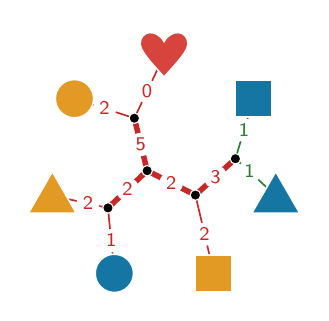
\begin{tikzpicture}[x=1.0cm,y=1.0cm,baseline=(current bounding box.center)]
\coordinate (v1) at (1.13770,0.90728);
\coordinate (v2) at (1.41868,-0.32381);
\coordinate (v3) at (-0.63137,-1.31106);
\coordinate (v4) at (0.63137,-1.31106);
\coordinate (v5) at (-1.41868,-0.32381);
\coordinate (v6) at (-1.13770,0.90728);
\coordinate (v7) at (0.00000,1.45517);
\coordinate (v8) at (-0.37733,0.65938);
\coordinate (v9) at (0.90613,0.14484);
\coordinate (v10) at (-0.71242,-0.47995);
\coordinate (v11) at (0.39817,-0.31682);
\coordinate (v12) at (-0.21455,-0.00744);
\draw[g2tree internal,draw=g2Barren] (v8)--(v12);
\draw[g2tree internal,draw=g2Barren] (v9)--(v11);
\draw[g2tree internal,draw=g2Barren] (v10)--(v12);
\draw[g2tree internal,draw=g2Barren] (v11)--(v12);
\draw[g2tree pendant,draw=g2Prime] (v1)--(v9);
\draw[g2tree pendant,draw=g2Prime] (v2)--(v9);
\draw[g2tree pendant,draw=g2Barren] (v3)--(v10);
\draw[g2tree pendant,draw=g2Barren] (v4)--(v11);
\draw[g2tree pendant,draw=g2Barren] (v5)--(v10);
\draw[g2tree pendant,draw=g2Barren] (v6)--(v8);
\draw[g2tree pendant,draw=g2Barren] (v7)--(v8);
\node[g2tree weight,text=g2Barren,font={\sffamily\fontsize{7.5}{8}\selectfont}] at (-0.29594,0.32597) {5};
\node[g2tree weight,text=g2Barren,font={\sffamily\fontsize{7.5}{8}\selectfont}] at (0.65215,-0.08599) {3};
\node[g2tree weight,text=g2Barren,font={\sffamily\fontsize{7.5}{8}\selectfont}] at (-0.46348,-0.24370) {2};
\node[g2tree weight,text=g2Barren,font={\sffamily\fontsize{7.5}{8}\selectfont}] at (0.09181,-0.16213) {2};
\node[g2tree weight,text=g2Prime,font={\sffamily\fontsize{7.5}{8}\selectfont}] at (1.01612,0.50700) {1};
\node[g2tree weight,text=g2Prime,font={\sffamily\fontsize{7.5}{8}\selectfont}] at (1.08552,-0.01919) {1};
\node[g2tree weight,text=g2Barren,font={\sffamily\fontsize{7.5}{8}\selectfont}] at (-0.67190,-0.89551) {1};
\node[g2tree weight,text=g2Barren,font={\sffamily\fontsize{7.5}{8}\selectfont}] at (0.51477,-0.81394) {2};
\node[g2tree weight,text=g2Barren,font={\sffamily\fontsize{7.5}{8}\selectfont}] at (-0.96595,-0.42390) {2};
\node[g2tree weight,text=g2Barren,font={\sffamily\fontsize{7.5}{8}\selectfont}] at (-0.75463,0.78239) {2};
\node[g2tree weight,text=g2Barren,font={\sffamily\fontsize{7.5}{8}\selectfont}] at (-0.21600,0.99962) {0};
\node[g2tree vertex] at (v8) {};
\node[g2tree vertex] at (v9) {};
\node[g2tree vertex] at (v10) {};
\node[g2tree vertex] at (v11) {};
\node[g2tree vertex] at (v12) {};
\node[g2tree dark,rectangle,minimum size=4.657500000000001mm,font={\sffamily\fontsize{9}{9}\selectfont\bfseries}] at (v1) {};
\begin{scope}[shift={(v2)},scale=1.0125000000000002,transform shape]
\path[fill=g2TaxonBlue,draw=white,line width=.55pt,line join=round] (0mm,3.0mm)--(-3.0mm,-2.2mm)--(3.0mm,-2.2mm)--cycle;
\end{scope}
\node[g2tree dark,circle,minimum size=4.86mm,font={\sffamily\fontsize{9}{9}\selectfont\bfseries}] at (v3) {};
\node[g2tree light,rectangle,minimum size=4.657500000000001mm,font={\sffamily\fontsize{9}{9}\selectfont\bfseries}] at (v4) {};
\begin{scope}[shift={(v5)},scale=1.0125000000000002,transform shape]
\path[fill=g2TaxonYellow,draw=white,line width=.55pt,line join=round] (0mm,3.0mm)--(-3.0mm,-2.2mm)--(3.0mm,-2.2mm)--cycle;
\end{scope}
\node[g2tree light,circle,minimum size=4.86mm,font={\sffamily\fontsize{9}{9}\selectfont\bfseries}] at (v6) {};
\begin{scope}[shift={(v7)},scale=1.0125000000000002,transform shape]
\path[fill=g2HeartRed,draw=white,line width=.55pt]
  (0mm,-2.7mm)..controls(-.45mm,-2.1mm)and(-3.0mm,.35mm)..(-3.0mm,1.45mm)
  ..controls(-3.0mm,3.2mm)and(-.9mm,3.4mm)..(0mm,1.75mm)
  ..controls(.9mm,3.4mm)and(3.0mm,3.2mm)..(3.0mm,1.45mm)
  ..controls(3.0mm,.35mm)and(.45mm,-2.1mm)..(0mm,-2.7mm)--cycle;
\end{scope}
\end{tikzpicture}
\endgroup
\par}
\end{minipage}
\\\noalign{\vskip 0.485cm}
\begin{minipage}[t]{\linewidth}
\noindent\textcolor{g2TreeRule}{\rule{\linewidth}{1pt}}\par
\noindent\textcolor[HTML]{000000}{\smash[b]{\textpdfrender{TextRenderingMode=FillStroke,LineWidth=.5pt}{\Large\bfseries\boldmath \oldstylenums{9}}{\large(12)}}}\hfill\textcolor{g2Prime}{\large2}\,\smash[b]{\tikz[baseline=0pt]\pic[scale=0.62] at (0,3.596mm) {g2apple};}\par
\vskip -1.2mm
{\centering
\begingroup
\definecolor{g2TaxonBlue}{HTML}{1676A3}
\definecolor{g2TaxonYellow}{HTML}{E39A24}
\definecolor{g2HeartRed}{HTML}{D7443E}
\tikzset{
  g2tree pendant/.style={draw=black,line width=.6pt,line cap=round},
  g2tree internal/.style={draw=black,line width=2pt,line cap=round},
  g2tree vertex/.style={circle,fill=black,draw=white,line width=.4pt,inner sep=0pt,minimum size=3.8pt},
  g2tree dark/.style={fill=g2TaxonBlue,draw=white,line width=.55pt,text=white,inner sep=0pt},
  g2tree light/.style={fill=g2TaxonYellow,draw=white,line width=.55pt,text=white,inner sep=0pt},
  g2tree weight/.style={circle,fill=white,draw=none,text=black,inner sep=.15pt,minimum size=8.5pt},
  g2tree aligned pendant/.style={fill=white,text=black,inner sep=.7pt,sloped,above=1pt,font={\sffamily\fontsize{7.5}{8}\selectfont}},
  g2tree aligned internal/.style={fill=white,text=black,inner sep=1pt,sloped,above=1pt,font={\sffamily\fontsize{7.5}{8}\selectfont\bfseries}},
}
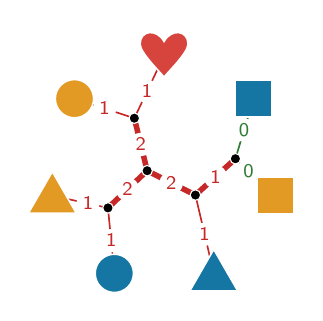
\begin{tikzpicture}[x=1.0cm,y=1.0cm,baseline=(current bounding box.center)]
\coordinate (v1) at (1.13770,0.90728);
\coordinate (v2) at (0.63137,-1.31106);
\coordinate (v3) at (-0.63137,-1.31106);
\coordinate (v4) at (1.41868,-0.32381);
\coordinate (v5) at (-1.41868,-0.32381);
\coordinate (v6) at (-1.13770,0.90728);
\coordinate (v7) at (0.00000,1.45517);
\coordinate (v8) at (-0.71242,-0.47995);
\coordinate (v9) at (-0.37733,0.65938);
\coordinate (v10) at (-0.21455,-0.00744);
\coordinate (v11) at (0.90613,0.14484);
\coordinate (v12) at (0.39817,-0.31682);
\draw[g2tree internal,draw=g2Barren] (v8)--(v10);
\draw[g2tree internal,draw=g2Barren] (v9)--(v10);
\draw[g2tree internal,draw=g2Barren] (v10)--(v12);
\draw[g2tree internal,draw=g2Barren] (v11)--(v12);
\draw[g2tree pendant,draw=g2Prime] (v1)--(v11);
\draw[g2tree pendant,draw=g2Barren] (v2)--(v12);
\draw[g2tree pendant,draw=g2Barren] (v3)--(v8);
\draw[g2tree pendant,draw=g2Prime] (v4)--(v11);
\draw[g2tree pendant,draw=g2Barren] (v5)--(v8);
\draw[g2tree pendant,draw=g2Barren] (v6)--(v9);
\draw[g2tree pendant,draw=g2Barren] (v7)--(v9);
\node[g2tree weight,text=g2Barren,font={\sffamily\fontsize{7.5}{8}\selectfont}] at (-0.46348,-0.24370) {2};
\node[g2tree weight,text=g2Barren,font={\sffamily\fontsize{7.5}{8}\selectfont}] at (-0.29594,0.32597) {2};
\node[g2tree weight,text=g2Barren,font={\sffamily\fontsize{7.5}{8}\selectfont}] at (0.09181,-0.16213) {2};
\node[g2tree weight,text=g2Barren,font={\sffamily\fontsize{7.5}{8}\selectfont}] at (0.65215,-0.08599) {1};
\node[g2tree weight,text=g2Prime,font={\sffamily\fontsize{7.5}{8}\selectfont}] at (1.01612,0.50700) {0};
\node[g2tree weight,text=g2Barren,font={\sffamily\fontsize{7.5}{8}\selectfont}] at (0.51477,-0.81394) {1};
\node[g2tree weight,text=g2Barren,font={\sffamily\fontsize{7.5}{8}\selectfont}] at (-0.67190,-0.89551) {1};
\node[g2tree weight,text=g2Prime,font={\sffamily\fontsize{7.5}{8}\selectfont}] at (1.07271,-0.00747) {0};
\node[g2tree weight,text=g2Barren,font={\sffamily\fontsize{7.5}{8}\selectfont}] at (-0.96595,-0.42390) {1};
\node[g2tree weight,text=g2Barren,font={\sffamily\fontsize{7.5}{8}\selectfont}] at (-0.75463,0.78239) {1};
\node[g2tree weight,text=g2Barren,font={\sffamily\fontsize{7.5}{8}\selectfont}] at (-0.21600,0.99962) {1};
\node[g2tree vertex] at (v8) {};
\node[g2tree vertex] at (v9) {};
\node[g2tree vertex] at (v10) {};
\node[g2tree vertex] at (v11) {};
\node[g2tree vertex] at (v12) {};
\node[g2tree dark,rectangle,minimum size=4.657500000000001mm,font={\sffamily\fontsize{9}{9}\selectfont\bfseries}] at (v1) {};
\begin{scope}[shift={(v2)},scale=1.0125000000000002,transform shape]
\path[fill=g2TaxonBlue,draw=white,line width=.55pt,line join=round] (0mm,3.0mm)--(-3.0mm,-2.2mm)--(3.0mm,-2.2mm)--cycle;
\end{scope}
\node[g2tree dark,circle,minimum size=4.86mm,font={\sffamily\fontsize{9}{9}\selectfont\bfseries}] at (v3) {};
\node[g2tree light,rectangle,minimum size=4.657500000000001mm,font={\sffamily\fontsize{9}{9}\selectfont\bfseries}] at (v4) {};
\begin{scope}[shift={(v5)},scale=1.0125000000000002,transform shape]
\path[fill=g2TaxonYellow,draw=white,line width=.55pt,line join=round] (0mm,3.0mm)--(-3.0mm,-2.2mm)--(3.0mm,-2.2mm)--cycle;
\end{scope}
\node[g2tree light,circle,minimum size=4.86mm,font={\sffamily\fontsize{9}{9}\selectfont\bfseries}] at (v6) {};
\begin{scope}[shift={(v7)},scale=1.0125000000000002,transform shape]
\path[fill=g2HeartRed,draw=white,line width=.55pt]
  (0mm,-2.7mm)..controls(-.45mm,-2.1mm)and(-3.0mm,.35mm)..(-3.0mm,1.45mm)
  ..controls(-3.0mm,3.2mm)and(-.9mm,3.4mm)..(0mm,1.75mm)
  ..controls(.9mm,3.4mm)and(3.0mm,3.2mm)..(3.0mm,1.45mm)
  ..controls(3.0mm,.35mm)and(.45mm,-2.1mm)..(0mm,-2.7mm)--cycle;
\end{scope}
\end{tikzpicture}
\endgroup
\par}
\end{minipage}
 & 
\begin{minipage}[t]{\linewidth}
\noindent\textcolor{g2TreeRule}{\rule{\linewidth}{1pt}}\par
\noindent\textcolor[HTML]{000000}{\smash[b]{\textpdfrender{TextRenderingMode=FillStroke,LineWidth=.5pt}{\Large\bfseries\boldmath \oldstylenums{10}}{\large(6)}}}\hfill\textcolor{g2Prime}{\large9}\,\smash[b]{\tikz[baseline=0pt]\pic[scale=0.62] at (0,3.596mm) {g2apple};}\par
\vskip -1.2mm
{\centering
\begingroup
\definecolor{g2TaxonBlue}{HTML}{1676A3}
\definecolor{g2TaxonYellow}{HTML}{E39A24}
\definecolor{g2HeartRed}{HTML}{D7443E}
\tikzset{
  g2tree pendant/.style={draw=black,line width=.6pt,line cap=round},
  g2tree internal/.style={draw=black,line width=2pt,line cap=round},
  g2tree vertex/.style={circle,fill=black,draw=white,line width=.4pt,inner sep=0pt,minimum size=3.8pt},
  g2tree dark/.style={fill=g2TaxonBlue,draw=white,line width=.55pt,text=white,inner sep=0pt},
  g2tree light/.style={fill=g2TaxonYellow,draw=white,line width=.55pt,text=white,inner sep=0pt},
  g2tree weight/.style={circle,fill=white,draw=none,text=black,inner sep=.15pt,minimum size=8.5pt},
  g2tree aligned pendant/.style={fill=white,text=black,inner sep=.7pt,sloped,above=1pt,font={\sffamily\fontsize{7.5}{8}\selectfont}},
  g2tree aligned internal/.style={fill=white,text=black,inner sep=1pt,sloped,above=1pt,font={\sffamily\fontsize{7.5}{8}\selectfont\bfseries}},
}
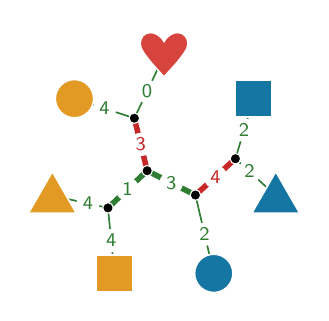
\begin{tikzpicture}[x=1.0cm,y=1.0cm,baseline=(current bounding box.center)]
\coordinate (v1) at (1.13770,0.90728);
\coordinate (v2) at (1.41868,-0.32381);
\coordinate (v3) at (0.63137,-1.31106);
\coordinate (v4) at (-0.63137,-1.31106);
\coordinate (v5) at (-1.41868,-0.32381);
\coordinate (v6) at (-1.13770,0.90728);
\coordinate (v7) at (0.00000,1.45517);
\coordinate (v8) at (0.90613,0.14484);
\coordinate (v9) at (0.39817,-0.31682);
\coordinate (v10) at (-0.37733,0.65938);
\coordinate (v11) at (-0.71242,-0.47995);
\coordinate (v12) at (-0.21455,-0.00744);
\draw[g2tree internal,draw=g2Barren] (v8)--(v9);
\draw[g2tree internal,draw=g2Prime] (v9)--(v12);
\draw[g2tree internal,draw=g2Barren] (v10)--(v12);
\draw[g2tree internal,draw=g2Prime] (v11)--(v12);
\draw[g2tree pendant,draw=g2Prime] (v1)--(v8);
\draw[g2tree pendant,draw=g2Prime] (v2)--(v8);
\draw[g2tree pendant,draw=g2Prime] (v3)--(v9);
\draw[g2tree pendant,draw=g2Prime] (v4)--(v11);
\draw[g2tree pendant,draw=g2Prime] (v5)--(v11);
\draw[g2tree pendant,draw=g2Prime] (v6)--(v10);
\draw[g2tree pendant,draw=g2Prime] (v7)--(v10);
\node[g2tree weight,text=g2Barren,font={\sffamily\fontsize{7.5}{8}\selectfont}] at (0.65215,-0.08599) {4};
\node[g2tree weight,text=g2Prime,font={\sffamily\fontsize{7.5}{8}\selectfont}] at (0.09181,-0.16213) {3};
\node[g2tree weight,text=g2Barren,font={\sffamily\fontsize{7.5}{8}\selectfont}] at (-0.29594,0.32597) {3};
\node[g2tree weight,text=g2Prime,font={\sffamily\fontsize{7.5}{8}\selectfont}] at (-0.46348,-0.24370) {1};
\node[g2tree weight,text=g2Prime,font={\sffamily\fontsize{7.5}{8}\selectfont}] at (1.01612,0.50700) {2};
\node[g2tree weight,text=g2Prime,font={\sffamily\fontsize{7.5}{8}\selectfont}] at (1.08552,-0.01919) {2};
\node[g2tree weight,text=g2Prime,font={\sffamily\fontsize{7.5}{8}\selectfont}] at (0.51477,-0.81394) {2};
\node[g2tree weight,text=g2Prime,font={\sffamily\fontsize{7.5}{8}\selectfont}] at (-0.67190,-0.89551) {4};
\node[g2tree weight,text=g2Prime,font={\sffamily\fontsize{7.5}{8}\selectfont}] at (-0.96595,-0.42390) {4};
\node[g2tree weight,text=g2Prime,font={\sffamily\fontsize{7.5}{8}\selectfont}] at (-0.75463,0.78239) {4};
\node[g2tree weight,text=g2Prime,font={\sffamily\fontsize{7.5}{8}\selectfont}] at (-0.21600,0.99962) {0};
\node[g2tree vertex] at (v8) {};
\node[g2tree vertex] at (v9) {};
\node[g2tree vertex] at (v10) {};
\node[g2tree vertex] at (v11) {};
\node[g2tree vertex] at (v12) {};
\node[g2tree dark,rectangle,minimum size=4.657500000000001mm,font={\sffamily\fontsize{9}{9}\selectfont\bfseries}] at (v1) {};
\begin{scope}[shift={(v2)},scale=1.0125000000000002,transform shape]
\path[fill=g2TaxonBlue,draw=white,line width=.55pt,line join=round] (0mm,3.0mm)--(-3.0mm,-2.2mm)--(3.0mm,-2.2mm)--cycle;
\end{scope}
\node[g2tree dark,circle,minimum size=4.86mm,font={\sffamily\fontsize{9}{9}\selectfont\bfseries}] at (v3) {};
\node[g2tree light,rectangle,minimum size=4.657500000000001mm,font={\sffamily\fontsize{9}{9}\selectfont\bfseries}] at (v4) {};
\begin{scope}[shift={(v5)},scale=1.0125000000000002,transform shape]
\path[fill=g2TaxonYellow,draw=white,line width=.55pt,line join=round] (0mm,3.0mm)--(-3.0mm,-2.2mm)--(3.0mm,-2.2mm)--cycle;
\end{scope}
\node[g2tree light,circle,minimum size=4.86mm,font={\sffamily\fontsize{9}{9}\selectfont\bfseries}] at (v6) {};
\begin{scope}[shift={(v7)},scale=1.0125000000000002,transform shape]
\path[fill=g2HeartRed,draw=white,line width=.55pt]
  (0mm,-2.7mm)..controls(-.45mm,-2.1mm)and(-3.0mm,.35mm)..(-3.0mm,1.45mm)
  ..controls(-3.0mm,3.2mm)and(-.9mm,3.4mm)..(0mm,1.75mm)
  ..controls(.9mm,3.4mm)and(3.0mm,3.2mm)..(3.0mm,1.45mm)
  ..controls(3.0mm,.35mm)and(.45mm,-2.1mm)..(0mm,-2.7mm)--cycle;
\end{scope}
\end{tikzpicture}
\endgroup
\par}
\end{minipage}
 & 
\begin{minipage}[t]{\linewidth}
\noindent\textcolor{g2TreeRule}{\rule{\linewidth}{1pt}}\par
\noindent\textcolor[HTML]{000000}{\smash[b]{\textpdfrender{TextRenderingMode=FillStroke,LineWidth=.5pt}{\Large\bfseries\boldmath \oldstylenums{11}}{\large(6)}}}\hfill\textcolor{g2Prime}{\large10}\,\smash[b]{\tikz[baseline=0pt]\pic[scale=0.62] at (0,3.596mm) {g2apple};}\par
\vskip -1.2mm
{\centering
\begingroup
\definecolor{g2TaxonBlue}{HTML}{1676A3}
\definecolor{g2TaxonYellow}{HTML}{E39A24}
\definecolor{g2HeartRed}{HTML}{D7443E}
\tikzset{
  g2tree pendant/.style={draw=black,line width=.6pt,line cap=round},
  g2tree internal/.style={draw=black,line width=2pt,line cap=round},
  g2tree vertex/.style={circle,fill=black,draw=white,line width=.4pt,inner sep=0pt,minimum size=3.8pt},
  g2tree dark/.style={fill=g2TaxonBlue,draw=white,line width=.55pt,text=white,inner sep=0pt},
  g2tree light/.style={fill=g2TaxonYellow,draw=white,line width=.55pt,text=white,inner sep=0pt},
  g2tree weight/.style={circle,fill=white,draw=none,text=black,inner sep=.15pt,minimum size=8.5pt},
  g2tree aligned pendant/.style={fill=white,text=black,inner sep=.7pt,sloped,above=1pt,font={\sffamily\fontsize{7.5}{8}\selectfont}},
  g2tree aligned internal/.style={fill=white,text=black,inner sep=1pt,sloped,above=1pt,font={\sffamily\fontsize{7.5}{8}\selectfont\bfseries}},
}
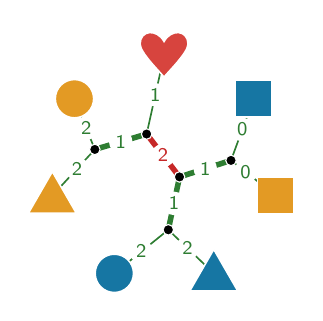
\begin{tikzpicture}[x=1.0cm,y=1.0cm,baseline=(current bounding box.center)]
\coordinate (v1) at (1.13770,0.90728);
\coordinate (v2) at (0.63137,-1.31106);
\coordinate (v3) at (-0.63137,-1.31106);
\coordinate (v4) at (1.41868,-0.32381);
\coordinate (v5) at (-1.41868,-0.32381);
\coordinate (v6) at (-1.13770,0.90728);
\coordinate (v7) at (0.00000,1.45517);
\coordinate (v8) at (-0.87924,0.26266);
\coordinate (v9) at (-0.22128,0.45821);
\coordinate (v10) at (0.85011,0.12332);
\coordinate (v11) at (0.05387,-0.75780);
\coordinate (v12) at (0.19653,-0.08639);
\draw[g2tree internal,draw=g2Prime] (v8)--(v9);
\draw[g2tree internal,draw=g2Barren] (v9)--(v12);
\draw[g2tree internal,draw=g2Prime] (v10)--(v12);
\draw[g2tree internal,draw=g2Prime] (v11)--(v12);
\draw[g2tree pendant,draw=g2Prime] (v1)--(v10);
\draw[g2tree pendant,draw=g2Prime] (v2)--(v11);
\draw[g2tree pendant,draw=g2Prime] (v3)--(v11);
\draw[g2tree pendant,draw=g2Prime] (v4)--(v10);
\draw[g2tree pendant,draw=g2Prime] (v5)--(v8);
\draw[g2tree pendant,draw=g2Prime] (v6)--(v8);
\draw[g2tree pendant,draw=g2Prime] (v7)--(v9);
\node[g2tree weight,text=g2Prime,font={\sffamily\fontsize{7.5}{8}\selectfont}] at (-0.55026,0.36043) {1};
\node[g2tree weight,text=g2Barren,font={\sffamily\fontsize{7.5}{8}\selectfont}] at (-0.01237,0.18591) {2};
\node[g2tree weight,text=g2Prime,font={\sffamily\fontsize{7.5}{8}\selectfont}] at (0.52332,0.01846) {1};
\node[g2tree weight,text=g2Prime,font={\sffamily\fontsize{7.5}{8}\selectfont}] at (0.12520,-0.42209) {1};
\node[g2tree weight,text=g2Prime,font={\sffamily\fontsize{7.5}{8}\selectfont}] at (0.99390,0.51530) {0};
\node[g2tree weight,text=g2Prime,font={\sffamily\fontsize{7.5}{8}\selectfont}] at (0.29656,-0.99030) {2};
\node[g2tree weight,text=g2Prime,font={\sffamily\fontsize{7.5}{8}\selectfont}] at (-0.28875,-1.03443) {2};
\node[g2tree weight,text=g2Prime,font={\sffamily\fontsize{7.5}{8}\selectfont}] at (1.03490,-0.02200) {0};
\node[g2tree weight,text=g2Prime,font={\sffamily\fontsize{7.5}{8}\selectfont}] at (-1.10479,0.01745) {2};
\node[g2tree weight,text=g2Prime,font={\sffamily\fontsize{7.5}{8}\selectfont}] at (-0.98775,0.53331) {2};
\node[g2tree weight,text=g2Prime,font={\sffamily\fontsize{7.5}{8}\selectfont}] at (-0.11064,0.95669) {1};
\node[g2tree vertex] at (v8) {};
\node[g2tree vertex] at (v9) {};
\node[g2tree vertex] at (v10) {};
\node[g2tree vertex] at (v11) {};
\node[g2tree vertex] at (v12) {};
\node[g2tree dark,rectangle,minimum size=4.657500000000001mm,font={\sffamily\fontsize{9}{9}\selectfont\bfseries}] at (v1) {};
\begin{scope}[shift={(v2)},scale=1.0125000000000002,transform shape]
\path[fill=g2TaxonBlue,draw=white,line width=.55pt,line join=round] (0mm,3.0mm)--(-3.0mm,-2.2mm)--(3.0mm,-2.2mm)--cycle;
\end{scope}
\node[g2tree dark,circle,minimum size=4.86mm,font={\sffamily\fontsize{9}{9}\selectfont\bfseries}] at (v3) {};
\node[g2tree light,rectangle,minimum size=4.657500000000001mm,font={\sffamily\fontsize{9}{9}\selectfont\bfseries}] at (v4) {};
\begin{scope}[shift={(v5)},scale=1.0125000000000002,transform shape]
\path[fill=g2TaxonYellow,draw=white,line width=.55pt,line join=round] (0mm,3.0mm)--(-3.0mm,-2.2mm)--(3.0mm,-2.2mm)--cycle;
\end{scope}
\node[g2tree light,circle,minimum size=4.86mm,font={\sffamily\fontsize{9}{9}\selectfont\bfseries}] at (v6) {};
\begin{scope}[shift={(v7)},scale=1.0125000000000002,transform shape]
\path[fill=g2HeartRed,draw=white,line width=.55pt]
  (0mm,-2.7mm)..controls(-.45mm,-2.1mm)and(-3.0mm,.35mm)..(-3.0mm,1.45mm)
  ..controls(-3.0mm,3.2mm)and(-.9mm,3.4mm)..(0mm,1.75mm)
  ..controls(.9mm,3.4mm)and(3.0mm,3.2mm)..(3.0mm,1.45mm)
  ..controls(3.0mm,.35mm)and(.45mm,-2.1mm)..(0mm,-2.7mm)--cycle;
\end{scope}
\end{tikzpicture}
\endgroup
\par}
\end{minipage}
 & 
\begin{minipage}[t]{\linewidth}
\noindent\textcolor{g2TreeRule}{\rule{\linewidth}{1pt}}\par
\noindent\textcolor[HTML]{000000}{\smash[b]{\textpdfrender{TextRenderingMode=FillStroke,LineWidth=.5pt}{\Large\bfseries\boldmath \oldstylenums{12}}{\large(6)}}}\hfill\textcolor{g2Prime}{\large10}\,\smash[b]{\tikz[baseline=0pt]\pic[scale=0.62] at (0,3.596mm) {g2apple};}\par
\vskip -1.2mm
{\centering
\begingroup
\definecolor{g2TaxonBlue}{HTML}{1676A3}
\definecolor{g2TaxonYellow}{HTML}{E39A24}
\definecolor{g2HeartRed}{HTML}{D7443E}
\tikzset{
  g2tree pendant/.style={draw=black,line width=.6pt,line cap=round},
  g2tree internal/.style={draw=black,line width=2pt,line cap=round},
  g2tree vertex/.style={circle,fill=black,draw=white,line width=.4pt,inner sep=0pt,minimum size=3.8pt},
  g2tree dark/.style={fill=g2TaxonBlue,draw=white,line width=.55pt,text=white,inner sep=0pt},
  g2tree light/.style={fill=g2TaxonYellow,draw=white,line width=.55pt,text=white,inner sep=0pt},
  g2tree weight/.style={circle,fill=white,draw=none,text=black,inner sep=.15pt,minimum size=8.5pt},
  g2tree aligned pendant/.style={fill=white,text=black,inner sep=.7pt,sloped,above=1pt,font={\sffamily\fontsize{7.5}{8}\selectfont}},
  g2tree aligned internal/.style={fill=white,text=black,inner sep=1pt,sloped,above=1pt,font={\sffamily\fontsize{7.5}{8}\selectfont\bfseries}},
}
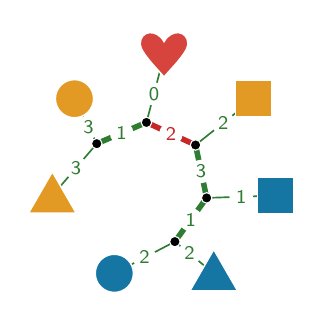
\begin{tikzpicture}[x=1.0cm,y=1.0cm,baseline=(current bounding box.center)]
\coordinate (v1) at (1.41868,-0.32381);
\coordinate (v2) at (0.63137,-1.31106);
\coordinate (v3) at (-0.63137,-1.31106);
\coordinate (v4) at (1.13770,0.90728);
\coordinate (v5) at (-1.41868,-0.32381);
\coordinate (v6) at (-1.13770,0.90728);
\coordinate (v7) at (0.00000,1.45517);
\coordinate (v8) at (0.13730,-0.90798);
\coordinate (v9) at (0.54092,-0.35279);
\coordinate (v10) at (0.40001,0.31899);
\coordinate (v11) at (-0.85466,0.33590);
\coordinate (v12) at (-0.22357,0.60586);
\draw[g2tree internal,draw=g2Prime] (v8)--(v9);
\draw[g2tree internal,draw=g2Prime] (v9)--(v10);
\draw[g2tree internal,draw=g2Barren] (v10)--(v12);
\draw[g2tree internal,draw=g2Prime] (v11)--(v12);
\draw[g2tree pendant,draw=g2Prime] (v1)--(v9);
\draw[g2tree pendant,draw=g2Prime] (v2)--(v8);
\draw[g2tree pendant,draw=g2Prime] (v3)--(v8);
\draw[g2tree pendant,draw=g2Prime] (v4)--(v10);
\draw[g2tree pendant,draw=g2Prime] (v5)--(v11);
\draw[g2tree pendant,draw=g2Prime] (v6)--(v11);
\draw[g2tree pendant,draw=g2Prime] (v7)--(v12);
\node[g2tree weight,text=g2Prime,font={\sffamily\fontsize{7.5}{8}\selectfont}] at (0.33911,-0.63038) {1};
\node[g2tree weight,text=g2Prime,font={\sffamily\fontsize{7.5}{8}\selectfont}] at (0.47046,-0.01690) {3};
\node[g2tree weight,text=g2Barren,font={\sffamily\fontsize{7.5}{8}\selectfont}] at (0.08822,0.46243) {2};
\node[g2tree weight,text=g2Prime,font={\sffamily\fontsize{7.5}{8}\selectfont}] at (-0.53912,0.47088) {1};
\node[g2tree weight,text=g2Prime,font={\sffamily\fontsize{7.5}{8}\selectfont}] at (0.97980,-0.33830) {1};
\node[g2tree weight,text=g2Prime,font={\sffamily\fontsize{7.5}{8}\selectfont}] at (0.32258,-1.05913) {2};
\node[g2tree weight,text=g2Prime,font={\sffamily\fontsize{7.5}{8}\selectfont}] at (-0.24704,-1.10952) {2};
\node[g2tree weight,text=g2Prime,font={\sffamily\fontsize{7.5}{8}\selectfont}] at (0.75041,0.59843) {2};
\node[g2tree weight,text=g2Prime,font={\sffamily\fontsize{7.5}{8}\selectfont}] at (-1.11738,0.02861) {3};
\node[g2tree weight,text=g2Prime,font={\sffamily\fontsize{7.5}{8}\selectfont}] at (-0.95885,0.54624) {3};
\node[g2tree weight,text=g2Prime,font={\sffamily\fontsize{7.5}{8}\selectfont}] at (-0.12835,0.96761) {0};
\node[g2tree vertex] at (v8) {};
\node[g2tree vertex] at (v9) {};
\node[g2tree vertex] at (v10) {};
\node[g2tree vertex] at (v11) {};
\node[g2tree vertex] at (v12) {};
\node[g2tree dark,rectangle,minimum size=4.657500000000001mm,font={\sffamily\fontsize{9}{9}\selectfont\bfseries}] at (v1) {};
\begin{scope}[shift={(v2)},scale=1.0125000000000002,transform shape]
\path[fill=g2TaxonBlue,draw=white,line width=.55pt,line join=round] (0mm,3.0mm)--(-3.0mm,-2.2mm)--(3.0mm,-2.2mm)--cycle;
\end{scope}
\node[g2tree dark,circle,minimum size=4.86mm,font={\sffamily\fontsize{9}{9}\selectfont\bfseries}] at (v3) {};
\node[g2tree light,rectangle,minimum size=4.657500000000001mm,font={\sffamily\fontsize{9}{9}\selectfont\bfseries}] at (v4) {};
\begin{scope}[shift={(v5)},scale=1.0125000000000002,transform shape]
\path[fill=g2TaxonYellow,draw=white,line width=.55pt,line join=round] (0mm,3.0mm)--(-3.0mm,-2.2mm)--(3.0mm,-2.2mm)--cycle;
\end{scope}
\node[g2tree light,circle,minimum size=4.86mm,font={\sffamily\fontsize{9}{9}\selectfont\bfseries}] at (v6) {};
\begin{scope}[shift={(v7)},scale=1.0125000000000002,transform shape]
\path[fill=g2HeartRed,draw=white,line width=.55pt]
  (0mm,-2.7mm)..controls(-.45mm,-2.1mm)and(-3.0mm,.35mm)..(-3.0mm,1.45mm)
  ..controls(-3.0mm,3.2mm)and(-.9mm,3.4mm)..(0mm,1.75mm)
  ..controls(.9mm,3.4mm)and(3.0mm,3.2mm)..(3.0mm,1.45mm)
  ..controls(3.0mm,.35mm)and(.45mm,-2.1mm)..(0mm,-2.7mm)--cycle;
\end{scope}
\end{tikzpicture}
\endgroup
\par}
\end{minipage}
\\\noalign{\vskip 0.485cm}
\begin{minipage}[t]{\linewidth}
\noindent\textcolor{g2TreeRule}{\rule{\linewidth}{1pt}}\par
\noindent\textcolor[HTML]{000000}{\smash[b]{\textpdfrender{TextRenderingMode=FillStroke,LineWidth=.5pt}{\Large\bfseries\boldmath \oldstylenums{13}}{\large(6)}}}\hfill\textcolor{g2Prime}{\large6}\,\smash[b]{\tikz[baseline=0pt]\pic[scale=0.62] at (0,3.596mm) {g2apple};}\par
\vskip -1.2mm
{\centering
\begingroup
\definecolor{g2TaxonBlue}{HTML}{1676A3}
\definecolor{g2TaxonYellow}{HTML}{E39A24}
\definecolor{g2HeartRed}{HTML}{D7443E}
\tikzset{
  g2tree pendant/.style={draw=black,line width=.6pt,line cap=round},
  g2tree internal/.style={draw=black,line width=2pt,line cap=round},
  g2tree vertex/.style={circle,fill=black,draw=white,line width=.4pt,inner sep=0pt,minimum size=3.8pt},
  g2tree dark/.style={fill=g2TaxonBlue,draw=white,line width=.55pt,text=white,inner sep=0pt},
  g2tree light/.style={fill=g2TaxonYellow,draw=white,line width=.55pt,text=white,inner sep=0pt},
  g2tree weight/.style={circle,fill=white,draw=none,text=black,inner sep=.15pt,minimum size=8.5pt},
  g2tree aligned pendant/.style={fill=white,text=black,inner sep=.7pt,sloped,above=1pt,font={\sffamily\fontsize{7.5}{8}\selectfont}},
  g2tree aligned internal/.style={fill=white,text=black,inner sep=1pt,sloped,above=1pt,font={\sffamily\fontsize{7.5}{8}\selectfont\bfseries}},
}
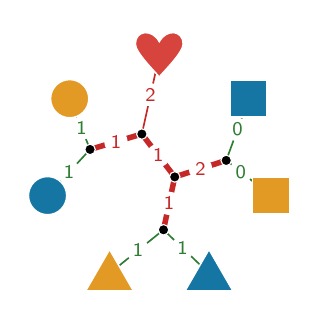
\begin{tikzpicture}[x=1.0cm,y=1.0cm,baseline=(current bounding box.center)]
\coordinate (v1) at (1.13770,0.90728);
\coordinate (v2) at (0.63137,-1.31106);
\coordinate (v3) at (-1.41868,-0.32381);
\coordinate (v4) at (1.41868,-0.32381);
\coordinate (v5) at (-0.63137,-1.31106);
\coordinate (v6) at (-1.13770,0.90728);
\coordinate (v7) at (0.00000,1.45517);
\coordinate (v8) at (0.85011,0.12332);
\coordinate (v9) at (0.05387,-0.75780);
\coordinate (v10) at (-0.87924,0.26266);
\coordinate (v11) at (-0.22128,0.45821);
\coordinate (v12) at (0.19653,-0.08639);
\draw[g2tree internal,draw=g2Barren] (v8)--(v12);
\draw[g2tree internal,draw=g2Barren] (v9)--(v12);
\draw[g2tree internal,draw=g2Barren] (v10)--(v11);
\draw[g2tree internal,draw=g2Barren] (v11)--(v12);
\draw[g2tree pendant,draw=g2Prime] (v1)--(v8);
\draw[g2tree pendant,draw=g2Prime] (v2)--(v9);
\draw[g2tree pendant,draw=g2Prime] (v3)--(v10);
\draw[g2tree pendant,draw=g2Prime] (v4)--(v8);
\draw[g2tree pendant,draw=g2Prime] (v5)--(v9);
\draw[g2tree pendant,draw=g2Prime] (v6)--(v10);
\draw[g2tree pendant,draw=g2Barren] (v7)--(v11);
\node[g2tree weight,text=g2Barren,font={\sffamily\fontsize{7.5}{8}\selectfont}] at (0.52332,0.01846) {2};
\node[g2tree weight,text=g2Barren,font={\sffamily\fontsize{7.5}{8}\selectfont}] at (0.12520,-0.42209) {1};
\node[g2tree weight,text=g2Barren,font={\sffamily\fontsize{7.5}{8}\selectfont}] at (-0.55026,0.36043) {1};
\node[g2tree weight,text=g2Barren,font={\sffamily\fontsize{7.5}{8}\selectfont}] at (-0.01237,0.18591) {1};
\node[g2tree weight,text=g2Prime,font={\sffamily\fontsize{7.5}{8}\selectfont}] at (0.99390,0.51530) {0};
\node[g2tree weight,text=g2Prime,font={\sffamily\fontsize{7.5}{8}\selectfont}] at (0.29656,-0.99030) {1};
\node[g2tree weight,text=g2Prime,font={\sffamily\fontsize{7.5}{8}\selectfont}] at (-1.14592,-0.02726) {1};
\node[g2tree weight,text=g2Prime,font={\sffamily\fontsize{7.5}{8}\selectfont}] at (1.03490,-0.02200) {0};
\node[g2tree weight,text=g2Prime,font={\sffamily\fontsize{7.5}{8}\selectfont}] at (-0.27062,-1.01979) {1};
\node[g2tree weight,text=g2Prime,font={\sffamily\fontsize{7.5}{8}\selectfont}] at (-0.98775,0.53331) {1};
\node[g2tree weight,text=g2Barren,font={\sffamily\fontsize{7.5}{8}\selectfont}] at (-0.11064,0.95669) {2};
\node[g2tree vertex] at (v8) {};
\node[g2tree vertex] at (v9) {};
\node[g2tree vertex] at (v10) {};
\node[g2tree vertex] at (v11) {};
\node[g2tree vertex] at (v12) {};
\node[g2tree dark,rectangle,minimum size=4.657500000000001mm,font={\sffamily\fontsize{9}{9}\selectfont\bfseries}] at (v1) {};
\begin{scope}[shift={(v2)},scale=1.0125000000000002,transform shape]
\path[fill=g2TaxonBlue,draw=white,line width=.55pt,line join=round] (0mm,3.0mm)--(-3.0mm,-2.2mm)--(3.0mm,-2.2mm)--cycle;
\end{scope}
\node[g2tree dark,circle,minimum size=4.86mm,font={\sffamily\fontsize{9}{9}\selectfont\bfseries}] at (v3) {};
\node[g2tree light,rectangle,minimum size=4.657500000000001mm,font={\sffamily\fontsize{9}{9}\selectfont\bfseries}] at (v4) {};
\begin{scope}[shift={(v5)},scale=1.0125000000000002,transform shape]
\path[fill=g2TaxonYellow,draw=white,line width=.55pt,line join=round] (0mm,3.0mm)--(-3.0mm,-2.2mm)--(3.0mm,-2.2mm)--cycle;
\end{scope}
\node[g2tree light,circle,minimum size=4.86mm,font={\sffamily\fontsize{9}{9}\selectfont\bfseries}] at (v6) {};
\begin{scope}[shift={(v7)},scale=1.0125000000000002,transform shape]
\path[fill=g2HeartRed,draw=white,line width=.55pt]
  (0mm,-2.7mm)..controls(-.45mm,-2.1mm)and(-3.0mm,.35mm)..(-3.0mm,1.45mm)
  ..controls(-3.0mm,3.2mm)and(-.9mm,3.4mm)..(0mm,1.75mm)
  ..controls(.9mm,3.4mm)and(3.0mm,3.2mm)..(3.0mm,1.45mm)
  ..controls(3.0mm,.35mm)and(.45mm,-2.1mm)..(0mm,-2.7mm)--cycle;
\end{scope}
\end{tikzpicture}
\endgroup
\par}
\end{minipage}
 & 
\begin{minipage}[t]{\linewidth}
\noindent\textcolor{g2TreeRule}{\rule{\linewidth}{1pt}}\par
\noindent\textcolor[HTML]{000000}{\smash[b]{\textpdfrender{TextRenderingMode=FillStroke,LineWidth=.5pt}{\Large\bfseries\boldmath \oldstylenums{14}}{\large(3)}}}\hfill\textcolor{g2Prime}{\large6}\,\smash[b]{\tikz[baseline=0pt]\pic[scale=0.62] at (0,3.596mm) {g2apple};}\par
\vskip -1.2mm
{\centering
\begingroup
\definecolor{g2TaxonBlue}{HTML}{1676A3}
\definecolor{g2TaxonYellow}{HTML}{E39A24}
\definecolor{g2HeartRed}{HTML}{D7443E}
\tikzset{
  g2tree pendant/.style={draw=black,line width=.6pt,line cap=round},
  g2tree internal/.style={draw=black,line width=2pt,line cap=round},
  g2tree vertex/.style={circle,fill=black,draw=white,line width=.4pt,inner sep=0pt,minimum size=3.8pt},
  g2tree dark/.style={fill=g2TaxonBlue,draw=white,line width=.55pt,text=white,inner sep=0pt},
  g2tree light/.style={fill=g2TaxonYellow,draw=white,line width=.55pt,text=white,inner sep=0pt},
  g2tree weight/.style={circle,fill=white,draw=none,text=black,inner sep=.15pt,minimum size=8.5pt},
  g2tree aligned pendant/.style={fill=white,text=black,inner sep=.7pt,sloped,above=1pt,font={\sffamily\fontsize{7.5}{8}\selectfont}},
  g2tree aligned internal/.style={fill=white,text=black,inner sep=1pt,sloped,above=1pt,font={\sffamily\fontsize{7.5}{8}\selectfont\bfseries}},
}
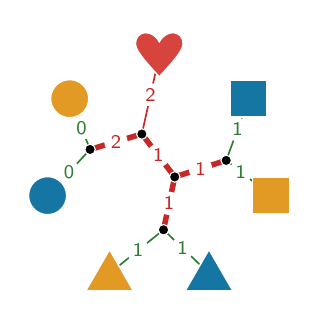
\begin{tikzpicture}[x=1.0cm,y=1.0cm,baseline=(current bounding box.center)]
\coordinate (v1) at (1.13770,0.90728);
\coordinate (v2) at (0.63137,-1.31106);
\coordinate (v3) at (-1.41868,-0.32381);
\coordinate (v4) at (1.41868,-0.32381);
\coordinate (v5) at (-0.63137,-1.31106);
\coordinate (v6) at (-1.13770,0.90728);
\coordinate (v7) at (0.00000,1.45517);
\coordinate (v8) at (-0.87924,0.26266);
\coordinate (v9) at (0.85011,0.12332);
\coordinate (v10) at (0.05387,-0.75780);
\coordinate (v11) at (-0.22128,0.45821);
\coordinate (v12) at (0.19653,-0.08639);
\draw[g2tree internal,draw=g2Barren] (v8)--(v11);
\draw[g2tree internal,draw=g2Barren] (v9)--(v12);
\draw[g2tree internal,draw=g2Barren] (v10)--(v12);
\draw[g2tree internal,draw=g2Barren] (v11)--(v12);
\draw[g2tree pendant,draw=g2Prime] (v1)--(v9);
\draw[g2tree pendant,draw=g2Prime] (v2)--(v10);
\draw[g2tree pendant,draw=g2Prime] (v3)--(v8);
\draw[g2tree pendant,draw=g2Prime] (v4)--(v9);
\draw[g2tree pendant,draw=g2Prime] (v5)--(v10);
\draw[g2tree pendant,draw=g2Prime] (v6)--(v8);
\draw[g2tree pendant,draw=g2Barren] (v7)--(v11);
\node[g2tree weight,text=g2Barren,font={\sffamily\fontsize{7.5}{8}\selectfont}] at (-0.55026,0.36043) {2};
\node[g2tree weight,text=g2Barren,font={\sffamily\fontsize{7.5}{8}\selectfont}] at (0.52332,0.01846) {1};
\node[g2tree weight,text=g2Barren,font={\sffamily\fontsize{7.5}{8}\selectfont}] at (0.12520,-0.42209) {1};
\node[g2tree weight,text=g2Barren,font={\sffamily\fontsize{7.5}{8}\selectfont}] at (-0.01237,0.18591) {1};
\node[g2tree weight,text=g2Prime,font={\sffamily\fontsize{7.5}{8}\selectfont}] at (0.99390,0.51530) {1};
\node[g2tree weight,text=g2Prime,font={\sffamily\fontsize{7.5}{8}\selectfont}] at (0.29656,-0.99030) {1};
\node[g2tree weight,text=g2Prime,font={\sffamily\fontsize{7.5}{8}\selectfont}] at (-1.14592,-0.02726) {0};
\node[g2tree weight,text=g2Prime,font={\sffamily\fontsize{7.5}{8}\selectfont}] at (1.03490,-0.02200) {1};
\node[g2tree weight,text=g2Prime,font={\sffamily\fontsize{7.5}{8}\selectfont}] at (-0.27062,-1.01979) {1};
\node[g2tree weight,text=g2Prime,font={\sffamily\fontsize{7.5}{8}\selectfont}] at (-0.98775,0.53331) {0};
\node[g2tree weight,text=g2Barren,font={\sffamily\fontsize{7.5}{8}\selectfont}] at (-0.11064,0.95669) {2};
\node[g2tree vertex] at (v8) {};
\node[g2tree vertex] at (v9) {};
\node[g2tree vertex] at (v10) {};
\node[g2tree vertex] at (v11) {};
\node[g2tree vertex] at (v12) {};
\node[g2tree dark,rectangle,minimum size=4.657500000000001mm,font={\sffamily\fontsize{9}{9}\selectfont\bfseries}] at (v1) {};
\begin{scope}[shift={(v2)},scale=1.0125000000000002,transform shape]
\path[fill=g2TaxonBlue,draw=white,line width=.55pt,line join=round] (0mm,3.0mm)--(-3.0mm,-2.2mm)--(3.0mm,-2.2mm)--cycle;
\end{scope}
\node[g2tree dark,circle,minimum size=4.86mm,font={\sffamily\fontsize{9}{9}\selectfont\bfseries}] at (v3) {};
\node[g2tree light,rectangle,minimum size=4.657500000000001mm,font={\sffamily\fontsize{9}{9}\selectfont\bfseries}] at (v4) {};
\begin{scope}[shift={(v5)},scale=1.0125000000000002,transform shape]
\path[fill=g2TaxonYellow,draw=white,line width=.55pt,line join=round] (0mm,3.0mm)--(-3.0mm,-2.2mm)--(3.0mm,-2.2mm)--cycle;
\end{scope}
\node[g2tree light,circle,minimum size=4.86mm,font={\sffamily\fontsize{9}{9}\selectfont\bfseries}] at (v6) {};
\begin{scope}[shift={(v7)},scale=1.0125000000000002,transform shape]
\path[fill=g2HeartRed,draw=white,line width=.55pt]
  (0mm,-2.7mm)..controls(-.45mm,-2.1mm)and(-3.0mm,.35mm)..(-3.0mm,1.45mm)
  ..controls(-3.0mm,3.2mm)and(-.9mm,3.4mm)..(0mm,1.75mm)
  ..controls(.9mm,3.4mm)and(3.0mm,3.2mm)..(3.0mm,1.45mm)
  ..controls(3.0mm,.35mm)and(.45mm,-2.1mm)..(0mm,-2.7mm)--cycle;
\end{scope}
\end{tikzpicture}
\endgroup
\par}
\end{minipage}
 & 
\begin{minipage}[t]{\linewidth}
\noindent\textcolor{g2TreeRule}{\rule{\linewidth}{1pt}}\par
\noindent\textcolor[HTML]{000000}{\smash[b]{\textpdfrender{TextRenderingMode=FillStroke,LineWidth=.5pt}{\Large\bfseries\boldmath \oldstylenums{15}}{\large(12)}}}\hfill\textcolor{g2Prime}{\large6}\,\smash[b]{\tikz[baseline=0pt]\pic[scale=0.62] at (0,3.596mm) {g2apple};}\par
\vskip -1.2mm
{\centering
\begingroup
\definecolor{g2TaxonBlue}{HTML}{1676A3}
\definecolor{g2TaxonYellow}{HTML}{E39A24}
\definecolor{g2HeartRed}{HTML}{D7443E}
\tikzset{
  g2tree pendant/.style={draw=black,line width=.6pt,line cap=round},
  g2tree internal/.style={draw=black,line width=2pt,line cap=round},
  g2tree vertex/.style={circle,fill=black,draw=white,line width=.4pt,inner sep=0pt,minimum size=3.8pt},
  g2tree dark/.style={fill=g2TaxonBlue,draw=white,line width=.55pt,text=white,inner sep=0pt},
  g2tree light/.style={fill=g2TaxonYellow,draw=white,line width=.55pt,text=white,inner sep=0pt},
  g2tree weight/.style={circle,fill=white,draw=none,text=black,inner sep=.15pt,minimum size=8.5pt},
  g2tree aligned pendant/.style={fill=white,text=black,inner sep=.7pt,sloped,above=1pt,font={\sffamily\fontsize{7.5}{8}\selectfont}},
  g2tree aligned internal/.style={fill=white,text=black,inner sep=1pt,sloped,above=1pt,font={\sffamily\fontsize{7.5}{8}\selectfont\bfseries}},
}
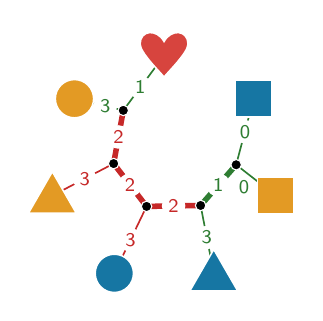
\begin{tikzpicture}[x=1.0cm,y=1.0cm,baseline=(current bounding box.center)]
\coordinate (v1) at (1.13770,0.90728);
\coordinate (v2) at (0.63137,-1.31106);
\coordinate (v3) at (-0.63137,-1.31106);
\coordinate (v4) at (1.41868,-0.32381);
\coordinate (v5) at (-1.41868,-0.32381);
\coordinate (v6) at (-1.13770,0.90728);
\coordinate (v7) at (0.00000,1.45517);
\coordinate (v8) at (-0.51766,0.75848);
\coordinate (v9) at (-0.64042,0.08315);
\coordinate (v10) at (-0.22199,-0.46096);
\coordinate (v11) at (0.91576,0.06818);
\coordinate (v12) at (0.46431,-0.44886);
\draw[g2tree internal,draw=g2Barren] (v8)--(v9);
\draw[g2tree internal,draw=g2Barren] (v9)--(v10);
\draw[g2tree internal,draw=g2Barren] (v10)--(v12);
\draw[g2tree internal,draw=g2Prime] (v11)--(v12);
\draw[g2tree pendant,draw=g2Prime] (v1)--(v11);
\draw[g2tree pendant,draw=g2Prime] (v2)--(v12);
\draw[g2tree pendant,draw=g2Barren] (v3)--(v10);
\draw[g2tree pendant,draw=g2Prime] (v4)--(v11);
\draw[g2tree pendant,draw=g2Barren] (v5)--(v9);
\draw[g2tree pendant,draw=g2Prime] (v6)--(v8);
\draw[g2tree pendant,draw=g2Prime] (v7)--(v8);
\node[g2tree weight,text=g2Barren,font={\sffamily\fontsize{7.5}{8}\selectfont}] at (-0.57904,0.42082) {2};
\node[g2tree weight,text=g2Barren,font={\sffamily\fontsize{7.5}{8}\selectfont}] at (-0.43120,-0.18890) {2};
\node[g2tree weight,text=g2Barren,font={\sffamily\fontsize{7.5}{8}\selectfont}] at (0.12116,-0.45491) {2};
\node[g2tree weight,text=g2Prime,font={\sffamily\fontsize{7.5}{8}\selectfont}] at (0.69004,-0.19034) {1};
\node[g2tree weight,text=g2Prime,font={\sffamily\fontsize{7.5}{8}\selectfont}] at (1.02673,0.48773) {0};
\node[g2tree weight,text=g2Prime,font={\sffamily\fontsize{7.5}{8}\selectfont}] at (0.54317,-0.85586) {3};
\node[g2tree weight,text=g2Barren,font={\sffamily\fontsize{7.5}{8}\selectfont}] at (-0.42668,-0.88601) {3};
\node[g2tree weight,text=g2Prime,font={\sffamily\fontsize{7.5}{8}\selectfont}] at (1.01430,-0.22028) {0};
\node[g2tree weight,text=g2Barren,font={\sffamily\fontsize{7.5}{8}\selectfont}] at (-1.00780,-0.10895) {3};
\node[g2tree weight,text=g2Prime,font={\sffamily\fontsize{7.5}{8}\selectfont}] at (-0.74591,0.81326) {3};
\node[g2tree weight,text=g2Prime,font={\sffamily\fontsize{7.5}{8}\selectfont}] at (-0.30069,1.05049) {1};
\node[g2tree vertex] at (v8) {};
\node[g2tree vertex] at (v9) {};
\node[g2tree vertex] at (v10) {};
\node[g2tree vertex] at (v11) {};
\node[g2tree vertex] at (v12) {};
\node[g2tree dark,rectangle,minimum size=4.657500000000001mm,font={\sffamily\fontsize{9}{9}\selectfont\bfseries}] at (v1) {};
\begin{scope}[shift={(v2)},scale=1.0125000000000002,transform shape]
\path[fill=g2TaxonBlue,draw=white,line width=.55pt,line join=round] (0mm,3.0mm)--(-3.0mm,-2.2mm)--(3.0mm,-2.2mm)--cycle;
\end{scope}
\node[g2tree dark,circle,minimum size=4.86mm,font={\sffamily\fontsize{9}{9}\selectfont\bfseries}] at (v3) {};
\node[g2tree light,rectangle,minimum size=4.657500000000001mm,font={\sffamily\fontsize{9}{9}\selectfont\bfseries}] at (v4) {};
\begin{scope}[shift={(v5)},scale=1.0125000000000002,transform shape]
\path[fill=g2TaxonYellow,draw=white,line width=.55pt,line join=round] (0mm,3.0mm)--(-3.0mm,-2.2mm)--(3.0mm,-2.2mm)--cycle;
\end{scope}
\node[g2tree light,circle,minimum size=4.86mm,font={\sffamily\fontsize{9}{9}\selectfont\bfseries}] at (v6) {};
\begin{scope}[shift={(v7)},scale=1.0125000000000002,transform shape]
\path[fill=g2HeartRed,draw=white,line width=.55pt]
  (0mm,-2.7mm)..controls(-.45mm,-2.1mm)and(-3.0mm,.35mm)..(-3.0mm,1.45mm)
  ..controls(-3.0mm,3.2mm)and(-.9mm,3.4mm)..(0mm,1.75mm)
  ..controls(.9mm,3.4mm)and(3.0mm,3.2mm)..(3.0mm,1.45mm)
  ..controls(3.0mm,.35mm)and(.45mm,-2.1mm)..(0mm,-2.7mm)--cycle;
\end{scope}
\end{tikzpicture}
\endgroup
\par}
\end{minipage}
 & 
\begin{minipage}[t]{\linewidth}
\noindent\textcolor{g2TreeRule}{\rule{\linewidth}{1pt}}\par
\noindent\textcolor[HTML]{000000}{\smash[b]{\textpdfrender{TextRenderingMode=FillStroke,LineWidth=.5pt}{\Large\bfseries\boldmath \oldstylenums{16}}{\large(12)}}}\hfill\textcolor{g2Prime}{\large6}\,\smash[b]{\tikz[baseline=0pt]\pic[scale=0.62] at (0,3.596mm) {g2apple};}\par
\vskip -1.2mm
{\centering
\begingroup
\definecolor{g2TaxonBlue}{HTML}{1676A3}
\definecolor{g2TaxonYellow}{HTML}{E39A24}
\definecolor{g2HeartRed}{HTML}{D7443E}
\tikzset{
  g2tree pendant/.style={draw=black,line width=.6pt,line cap=round},
  g2tree internal/.style={draw=black,line width=2pt,line cap=round},
  g2tree vertex/.style={circle,fill=black,draw=white,line width=.4pt,inner sep=0pt,minimum size=3.8pt},
  g2tree dark/.style={fill=g2TaxonBlue,draw=white,line width=.55pt,text=white,inner sep=0pt},
  g2tree light/.style={fill=g2TaxonYellow,draw=white,line width=.55pt,text=white,inner sep=0pt},
  g2tree weight/.style={circle,fill=white,draw=none,text=black,inner sep=.15pt,minimum size=8.5pt},
  g2tree aligned pendant/.style={fill=white,text=black,inner sep=.7pt,sloped,above=1pt,font={\sffamily\fontsize{7.5}{8}\selectfont}},
  g2tree aligned internal/.style={fill=white,text=black,inner sep=1pt,sloped,above=1pt,font={\sffamily\fontsize{7.5}{8}\selectfont\bfseries}},
}
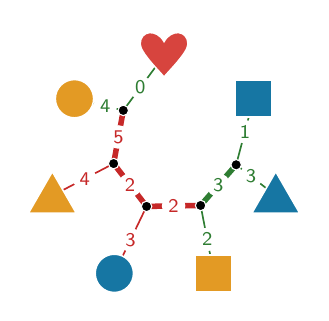
\begin{tikzpicture}[x=1.0cm,y=1.0cm,baseline=(current bounding box.center)]
\coordinate (v1) at (1.13770,0.90728);
\coordinate (v2) at (1.41868,-0.32381);
\coordinate (v3) at (-0.63137,-1.31106);
\coordinate (v4) at (0.63137,-1.31106);
\coordinate (v5) at (-1.41868,-0.32381);
\coordinate (v6) at (-1.13770,0.90728);
\coordinate (v7) at (0.00000,1.45517);
\coordinate (v8) at (-0.51766,0.75848);
\coordinate (v9) at (0.91576,0.06818);
\coordinate (v10) at (0.46431,-0.44886);
\coordinate (v11) at (-0.22199,-0.46096);
\coordinate (v12) at (-0.64042,0.08315);
\draw[g2tree internal,draw=g2Barren] (v8)--(v12);
\draw[g2tree internal,draw=g2Prime] (v9)--(v10);
\draw[g2tree internal,draw=g2Barren] (v10)--(v11);
\draw[g2tree internal,draw=g2Barren] (v11)--(v12);
\draw[g2tree pendant,draw=g2Prime] (v1)--(v9);
\draw[g2tree pendant,draw=g2Prime] (v2)--(v9);
\draw[g2tree pendant,draw=g2Barren] (v3)--(v11);
\draw[g2tree pendant,draw=g2Prime] (v4)--(v10);
\draw[g2tree pendant,draw=g2Barren] (v5)--(v12);
\draw[g2tree pendant,draw=g2Prime] (v6)--(v8);
\draw[g2tree pendant,draw=g2Prime] (v7)--(v8);
\node[g2tree weight,text=g2Barren,font={\sffamily\fontsize{7.5}{8}\selectfont}] at (-0.57904,0.42082) {5};
\node[g2tree weight,text=g2Prime,font={\sffamily\fontsize{7.5}{8}\selectfont}] at (0.69004,-0.19034) {3};
\node[g2tree weight,text=g2Barren,font={\sffamily\fontsize{7.5}{8}\selectfont}] at (0.12116,-0.45491) {2};
\node[g2tree weight,text=g2Barren,font={\sffamily\fontsize{7.5}{8}\selectfont}] at (-0.43120,-0.18890) {2};
\node[g2tree weight,text=g2Prime,font={\sffamily\fontsize{7.5}{8}\selectfont}] at (1.02673,0.48773) {1};
\node[g2tree weight,text=g2Prime,font={\sffamily\fontsize{7.5}{8}\selectfont}] at (1.10436,-0.07881) {3};
\node[g2tree weight,text=g2Barren,font={\sffamily\fontsize{7.5}{8}\selectfont}] at (-0.42668,-0.88601) {3};
\node[g2tree weight,text=g2Prime,font={\sffamily\fontsize{7.5}{8}\selectfont}] at (0.54784,-0.87996) {2};
\node[g2tree weight,text=g2Barren,font={\sffamily\fontsize{7.5}{8}\selectfont}] at (-1.00780,-0.10895) {4};
\node[g2tree weight,text=g2Prime,font={\sffamily\fontsize{7.5}{8}\selectfont}] at (-0.74591,0.81326) {4};
\node[g2tree weight,text=g2Prime,font={\sffamily\fontsize{7.5}{8}\selectfont}] at (-0.30069,1.05049) {0};
\node[g2tree vertex] at (v8) {};
\node[g2tree vertex] at (v9) {};
\node[g2tree vertex] at (v10) {};
\node[g2tree vertex] at (v11) {};
\node[g2tree vertex] at (v12) {};
\node[g2tree dark,rectangle,minimum size=4.657500000000001mm,font={\sffamily\fontsize{9}{9}\selectfont\bfseries}] at (v1) {};
\begin{scope}[shift={(v2)},scale=1.0125000000000002,transform shape]
\path[fill=g2TaxonBlue,draw=white,line width=.55pt,line join=round] (0mm,3.0mm)--(-3.0mm,-2.2mm)--(3.0mm,-2.2mm)--cycle;
\end{scope}
\node[g2tree dark,circle,minimum size=4.86mm,font={\sffamily\fontsize{9}{9}\selectfont\bfseries}] at (v3) {};
\node[g2tree light,rectangle,minimum size=4.657500000000001mm,font={\sffamily\fontsize{9}{9}\selectfont\bfseries}] at (v4) {};
\begin{scope}[shift={(v5)},scale=1.0125000000000002,transform shape]
\path[fill=g2TaxonYellow,draw=white,line width=.55pt,line join=round] (0mm,3.0mm)--(-3.0mm,-2.2mm)--(3.0mm,-2.2mm)--cycle;
\end{scope}
\node[g2tree light,circle,minimum size=4.86mm,font={\sffamily\fontsize{9}{9}\selectfont\bfseries}] at (v6) {};
\begin{scope}[shift={(v7)},scale=1.0125000000000002,transform shape]
\path[fill=g2HeartRed,draw=white,line width=.55pt]
  (0mm,-2.7mm)..controls(-.45mm,-2.1mm)and(-3.0mm,.35mm)..(-3.0mm,1.45mm)
  ..controls(-3.0mm,3.2mm)and(-.9mm,3.4mm)..(0mm,1.75mm)
  ..controls(.9mm,3.4mm)and(3.0mm,3.2mm)..(3.0mm,1.45mm)
  ..controls(3.0mm,.35mm)and(.45mm,-2.1mm)..(0mm,-2.7mm)--cycle;
\end{scope}
\end{tikzpicture}
\endgroup
\par}
\end{minipage}
\\\noalign{\vskip 0.485cm}
\multicolumn{1}{@{}p{3.9cm}@{\hspace{\dimexpr0.11cm-1pt/2\relax}{\color{g2TreeRule}\vrule width 1pt height 1pt}\hspace{\dimexpr0.11cm-1pt/2\relax}}}{%
\begin{minipage}[t]{\linewidth}
\noindent\textcolor{g2TreeRule}{\rule{\linewidth}{1pt}}\par
\noindent\textcolor[HTML]{000000}{\smash[b]{\textpdfrender{TextRenderingMode=FillStroke,LineWidth=.5pt}{\Large\bfseries\boldmath \oldstylenums{17}}{\large(12)}}}\hfill\textcolor{g2Prime}{\large8}\,\smash[b]{\tikz[baseline=0pt]\pic[scale=0.62] at (0,3.596mm) {g2apple};}\par
\vskip -1.2mm
{\centering
\begingroup
\definecolor{g2TaxonBlue}{HTML}{1676A3}
\definecolor{g2TaxonYellow}{HTML}{E39A24}
\definecolor{g2HeartRed}{HTML}{D7443E}
\tikzset{
  g2tree pendant/.style={draw=black,line width=.6pt,line cap=round},
  g2tree internal/.style={draw=black,line width=2pt,line cap=round},
  g2tree vertex/.style={circle,fill=black,draw=white,line width=.4pt,inner sep=0pt,minimum size=3.8pt},
  g2tree dark/.style={fill=g2TaxonBlue,draw=white,line width=.55pt,text=white,inner sep=0pt},
  g2tree light/.style={fill=g2TaxonYellow,draw=white,line width=.55pt,text=white,inner sep=0pt},
  g2tree weight/.style={circle,fill=white,draw=none,text=black,inner sep=.15pt,minimum size=8.5pt},
  g2tree aligned pendant/.style={fill=white,text=black,inner sep=.7pt,sloped,above=1pt,font={\sffamily\fontsize{7.5}{8}\selectfont}},
  g2tree aligned internal/.style={fill=white,text=black,inner sep=1pt,sloped,above=1pt,font={\sffamily\fontsize{7.5}{8}\selectfont\bfseries}},
}
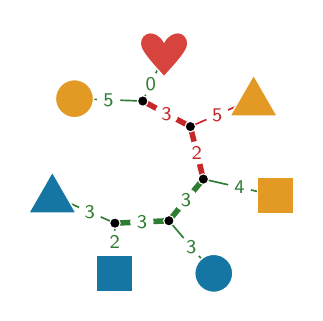
\begin{tikzpicture}[x=1.0cm,y=1.0cm,baseline=(current bounding box.center)]
\coordinate (v1) at (-0.63137,-1.31106);
\coordinate (v2) at (-1.41868,-0.32381);
\coordinate (v3) at (0.63137,-1.31106);
\coordinate (v4) at (1.41868,-0.32381);
\coordinate (v5) at (1.13770,0.90728);
\coordinate (v6) at (-1.13770,0.90728);
\coordinate (v7) at (0.00000,1.45517);
\coordinate (v8) at (-0.62428,-0.67346);
\coordinate (v9) at (0.06144,-0.64287);
\coordinate (v10) at (-0.27025,0.87763);
\coordinate (v11) at (0.49880,-0.11385);
\coordinate (v12) at (0.33429,0.55255);
\draw[g2tree internal,draw=g2Prime] (v8)--(v9);
\draw[g2tree internal,draw=g2Prime] (v9)--(v11);
\draw[g2tree internal,draw=g2Barren] (v10)--(v12);
\draw[g2tree internal,draw=g2Barren] (v11)--(v12);
\draw[g2tree pendant,draw=g2Prime] (v1)--(v8);
\draw[g2tree pendant,draw=g2Prime] (v2)--(v8);
\draw[g2tree pendant,draw=g2Prime] (v3)--(v9);
\draw[g2tree pendant,draw=g2Prime] (v4)--(v11);
\draw[g2tree pendant,draw=g2Barren] (v5)--(v12);
\draw[g2tree pendant,draw=g2Prime] (v6)--(v10);
\draw[g2tree pendant,draw=g2Prime] (v7)--(v10);
\node[g2tree weight,text=g2Prime,font={\sffamily\fontsize{7.5}{8}\selectfont}] at (-0.28142,-0.65816) {3};
\node[g2tree weight,text=g2Prime,font={\sffamily\fontsize{7.5}{8}\selectfont}] at (0.28012,-0.37836) {3};
\node[g2tree weight,text=g2Barren,font={\sffamily\fontsize{7.5}{8}\selectfont}] at (0.03202,0.71509) {3};
\node[g2tree weight,text=g2Barren,font={\sffamily\fontsize{7.5}{8}\selectfont}] at (0.41654,0.21935) {2};
\node[g2tree weight,text=g2Prime,font={\sffamily\fontsize{7.5}{8}\selectfont}] at (-0.62700,-0.91830) {2};
\node[g2tree weight,text=g2Prime,font={\sffamily\fontsize{7.5}{8}\selectfont}] at (-0.94204,-0.53360) {3};
\node[g2tree weight,text=g2Prime,font={\sffamily\fontsize{7.5}{8}\selectfont}] at (0.34641,-0.97696) {3};
\node[g2tree weight,text=g2Prime,font={\sffamily\fontsize{7.5}{8}\selectfont}] at (0.95874,-0.21883) {4};
\node[g2tree weight,text=g2Barren,font={\sffamily\fontsize{7.5}{8}\selectfont}] at (0.67574,0.70331) {5};
\node[g2tree weight,text=g2Prime,font={\sffamily\fontsize{7.5}{8}\selectfont}] at (-0.70397,0.89246) {5};
\node[g2tree weight,text=g2Prime,font={\sffamily\fontsize{7.5}{8}\selectfont}] at (-0.16891,1.09421) {0};
\node[g2tree vertex] at (v8) {};
\node[g2tree vertex] at (v9) {};
\node[g2tree vertex] at (v10) {};
\node[g2tree vertex] at (v11) {};
\node[g2tree vertex] at (v12) {};
\node[g2tree dark,rectangle,minimum size=4.657500000000001mm,font={\sffamily\fontsize{9}{9}\selectfont\bfseries}] at (v1) {};
\begin{scope}[shift={(v2)},scale=1.0125000000000002,transform shape]
\path[fill=g2TaxonBlue,draw=white,line width=.55pt,line join=round] (0mm,3.0mm)--(-3.0mm,-2.2mm)--(3.0mm,-2.2mm)--cycle;
\end{scope}
\node[g2tree dark,circle,minimum size=4.86mm,font={\sffamily\fontsize{9}{9}\selectfont\bfseries}] at (v3) {};
\node[g2tree light,rectangle,minimum size=4.657500000000001mm,font={\sffamily\fontsize{9}{9}\selectfont\bfseries}] at (v4) {};
\begin{scope}[shift={(v5)},scale=1.0125000000000002,transform shape]
\path[fill=g2TaxonYellow,draw=white,line width=.55pt,line join=round] (0mm,3.0mm)--(-3.0mm,-2.2mm)--(3.0mm,-2.2mm)--cycle;
\end{scope}
\node[g2tree light,circle,minimum size=4.86mm,font={\sffamily\fontsize{9}{9}\selectfont\bfseries}] at (v6) {};
\begin{scope}[shift={(v7)},scale=1.0125000000000002,transform shape]
\path[fill=g2HeartRed,draw=white,line width=.55pt]
  (0mm,-2.7mm)..controls(-.45mm,-2.1mm)and(-3.0mm,.35mm)..(-3.0mm,1.45mm)
  ..controls(-3.0mm,3.2mm)and(-.9mm,3.4mm)..(0mm,1.75mm)
  ..controls(.9mm,3.4mm)and(3.0mm,3.2mm)..(3.0mm,1.45mm)
  ..controls(3.0mm,.35mm)and(.45mm,-2.1mm)..(0mm,-2.7mm)--cycle;
\end{scope}
\end{tikzpicture}
\endgroup
\par}
\end{minipage}}
 & 
\begin{minipage}[t]{\linewidth}
\noindent\textcolor{g2TreeRule}{\rule{\linewidth}{1pt}}\par
\noindent\textcolor[HTML]{000000}{\smash[b]{\textpdfrender{TextRenderingMode=FillStroke,LineWidth=.5pt}{\Large\bfseries\boldmath \oldstylenums{18}}{\large(6)}}}\hfill\textcolor{g2Prime}{\large2}\,\smash[b]{\tikz[baseline=0pt]\pic[scale=0.62] at (0,3.596mm) {g2apple};}\par
\vskip -1.2mm
{\centering
\begingroup
\definecolor{g2TaxonBlue}{HTML}{1676A3}
\definecolor{g2TaxonYellow}{HTML}{E39A24}
\definecolor{g2HeartRed}{HTML}{D7443E}
\tikzset{
  g2tree pendant/.style={draw=black,line width=.6pt,line cap=round},
  g2tree internal/.style={draw=black,line width=2pt,line cap=round},
  g2tree vertex/.style={circle,fill=black,draw=white,line width=.4pt,inner sep=0pt,minimum size=3.8pt},
  g2tree dark/.style={fill=g2TaxonBlue,draw=white,line width=.55pt,text=white,inner sep=0pt},
  g2tree light/.style={fill=g2TaxonYellow,draw=white,line width=.55pt,text=white,inner sep=0pt},
  g2tree weight/.style={circle,fill=white,draw=none,text=black,inner sep=.15pt,minimum size=8.5pt},
  g2tree aligned pendant/.style={fill=white,text=black,inner sep=.7pt,sloped,above=1pt,font={\sffamily\fontsize{7.5}{8}\selectfont}},
  g2tree aligned internal/.style={fill=white,text=black,inner sep=1pt,sloped,above=1pt,font={\sffamily\fontsize{7.5}{8}\selectfont\bfseries}},
}
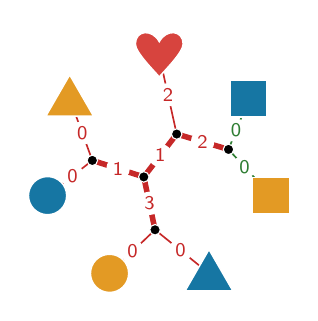
\begin{tikzpicture}[x=1.0cm,y=1.0cm,baseline=(current bounding box.center)]
\coordinate (v1) at (1.13770,0.90728);
\coordinate (v2) at (0.63137,-1.31106);
\coordinate (v3) at (-1.41868,-0.32381);
\coordinate (v4) at (1.41868,-0.32381);
\coordinate (v5) at (-1.13770,0.90728);
\coordinate (v6) at (-0.63137,-1.31106);
\coordinate (v7) at (0.00000,1.45517);
\coordinate (v8) at (-0.05387,-0.75780);
\coordinate (v9) at (0.87924,0.26266);
\coordinate (v10) at (-0.85011,0.12332);
\coordinate (v11) at (0.22128,0.45821);
\coordinate (v12) at (-0.19653,-0.08639);
\draw[g2tree internal,draw=g2Barren] (v8)--(v12);
\draw[g2tree internal,draw=g2Barren] (v9)--(v11);
\draw[g2tree internal,draw=g2Barren] (v10)--(v12);
\draw[g2tree internal,draw=g2Barren] (v11)--(v12);
\draw[g2tree pendant,draw=g2Prime] (v1)--(v9);
\draw[g2tree pendant,draw=g2Barren] (v2)--(v8);
\draw[g2tree pendant,draw=g2Barren] (v3)--(v10);
\draw[g2tree pendant,draw=g2Prime] (v4)--(v9);
\draw[g2tree pendant,draw=g2Barren] (v5)--(v10);
\draw[g2tree pendant,draw=g2Barren] (v6)--(v8);
\draw[g2tree pendant,draw=g2Barren] (v7)--(v11);
\node[g2tree weight,text=g2Barren,font={\sffamily\fontsize{7.5}{8}\selectfont}] at (-0.12520,-0.42209) {3};
\node[g2tree weight,text=g2Barren,font={\sffamily\fontsize{7.5}{8}\selectfont}] at (0.55026,0.36043) {2};
\node[g2tree weight,text=g2Barren,font={\sffamily\fontsize{7.5}{8}\selectfont}] at (-0.52332,0.01846) {1};
\node[g2tree weight,text=g2Barren,font={\sffamily\fontsize{7.5}{8}\selectfont}] at (0.01237,0.18591) {1};
\node[g2tree weight,text=g2Prime,font={\sffamily\fontsize{7.5}{8}\selectfont}] at (0.97616,0.50439) {0};
\node[g2tree weight,text=g2Barren,font={\sffamily\fontsize{7.5}{8}\selectfont}] at (0.27062,-1.01979) {0};
\node[g2tree weight,text=g2Barren,font={\sffamily\fontsize{7.5}{8}\selectfont}] at (-1.10197,-0.07474) {0};
\node[g2tree weight,text=g2Prime,font={\sffamily\fontsize{7.5}{8}\selectfont}] at (1.08153,0.04274) {0};
\node[g2tree weight,text=g2Barren,font={\sffamily\fontsize{7.5}{8}\selectfont}] at (-0.97801,0.47198) {0};
\node[g2tree weight,text=g2Barren,font={\sffamily\fontsize{7.5}{8}\selectfont}] at (-0.34043,-1.03233) {0};
\node[g2tree weight,text=g2Barren,font={\sffamily\fontsize{7.5}{8}\selectfont}] at (0.11064,0.95669) {2};
\node[g2tree vertex] at (v8) {};
\node[g2tree vertex] at (v9) {};
\node[g2tree vertex] at (v10) {};
\node[g2tree vertex] at (v11) {};
\node[g2tree vertex] at (v12) {};
\node[g2tree dark,rectangle,minimum size=4.657500000000001mm,font={\sffamily\fontsize{9}{9}\selectfont\bfseries}] at (v1) {};
\begin{scope}[shift={(v2)},scale=1.0125000000000002,transform shape]
\path[fill=g2TaxonBlue,draw=white,line width=.55pt,line join=round] (0mm,3.0mm)--(-3.0mm,-2.2mm)--(3.0mm,-2.2mm)--cycle;
\end{scope}
\node[g2tree dark,circle,minimum size=4.86mm,font={\sffamily\fontsize{9}{9}\selectfont\bfseries}] at (v3) {};
\node[g2tree light,rectangle,minimum size=4.657500000000001mm,font={\sffamily\fontsize{9}{9}\selectfont\bfseries}] at (v4) {};
\begin{scope}[shift={(v5)},scale=1.0125000000000002,transform shape]
\path[fill=g2TaxonYellow,draw=white,line width=.55pt,line join=round] (0mm,3.0mm)--(-3.0mm,-2.2mm)--(3.0mm,-2.2mm)--cycle;
\end{scope}
\node[g2tree light,circle,minimum size=4.86mm,font={\sffamily\fontsize{9}{9}\selectfont\bfseries}] at (v6) {};
\begin{scope}[shift={(v7)},scale=1.0125000000000002,transform shape]
\path[fill=g2HeartRed,draw=white,line width=.55pt]
  (0mm,-2.7mm)..controls(-.45mm,-2.1mm)and(-3.0mm,.35mm)..(-3.0mm,1.45mm)
  ..controls(-3.0mm,3.2mm)and(-.9mm,3.4mm)..(0mm,1.75mm)
  ..controls(.9mm,3.4mm)and(3.0mm,3.2mm)..(3.0mm,1.45mm)
  ..controls(3.0mm,.35mm)and(.45mm,-2.1mm)..(0mm,-2.7mm)--cycle;
\end{scope}
\end{tikzpicture}
\endgroup
\par}
\vskip 0pt plus 1filll
\noindent\rlap{char\ 2}\par
\end{minipage}
 & 
\begin{minipage}[t]{\linewidth}
\noindent\textcolor{g2TreeRule}{\rule{\linewidth}{1pt}}\par
\noindent\textcolor[HTML]{000000}{\smash[b]{\textpdfrender{TextRenderingMode=FillStroke,LineWidth=.5pt}{\Large\bfseries\boldmath \oldstylenums{19}}{\large(3)}}}\hfill\textcolor{g2Prime}{\large0}\,\smash[b]{\tikz[baseline=0pt]\pic[scale=0.62] at (0,3.596mm) {g2apple};}\par
\vskip -1.2mm
{\centering
\begingroup
\definecolor{g2TaxonBlue}{HTML}{1676A3}
\definecolor{g2TaxonYellow}{HTML}{E39A24}
\definecolor{g2HeartRed}{HTML}{D7443E}
\tikzset{
  g2tree pendant/.style={draw=black,line width=.6pt,line cap=round},
  g2tree internal/.style={draw=black,line width=2pt,line cap=round},
  g2tree vertex/.style={circle,fill=black,draw=white,line width=.4pt,inner sep=0pt,minimum size=3.8pt},
  g2tree dark/.style={fill=g2TaxonBlue,draw=white,line width=.55pt,text=white,inner sep=0pt},
  g2tree light/.style={fill=g2TaxonYellow,draw=white,line width=.55pt,text=white,inner sep=0pt},
  g2tree weight/.style={circle,fill=white,draw=none,text=black,inner sep=.15pt,minimum size=8.5pt},
  g2tree aligned pendant/.style={fill=white,text=black,inner sep=.7pt,sloped,above=1pt,font={\sffamily\fontsize{7.5}{8}\selectfont}},
  g2tree aligned internal/.style={fill=white,text=black,inner sep=1pt,sloped,above=1pt,font={\sffamily\fontsize{7.5}{8}\selectfont\bfseries}},
}
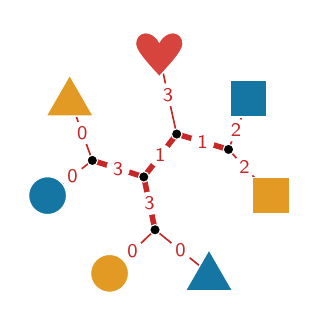
\begin{tikzpicture}[x=1.0cm,y=1.0cm,baseline=(current bounding box.center)]
\coordinate (v1) at (1.13770,0.90728);
\coordinate (v2) at (0.63137,-1.31106);
\coordinate (v3) at (-1.41868,-0.32381);
\coordinate (v4) at (1.41868,-0.32381);
\coordinate (v5) at (-1.13770,0.90728);
\coordinate (v6) at (-0.63137,-1.31106);
\coordinate (v7) at (0.00000,1.45517);
\coordinate (v8) at (-0.05387,-0.75780);
\coordinate (v9) at (-0.85011,0.12332);
\coordinate (v10) at (0.87924,0.26266);
\coordinate (v11) at (0.22128,0.45821);
\coordinate (v12) at (-0.19653,-0.08639);
\draw[g2tree internal,draw=g2Barren] (v8)--(v12);
\draw[g2tree internal,draw=g2Barren] (v9)--(v12);
\draw[g2tree internal,draw=g2Barren] (v10)--(v11);
\draw[g2tree internal,draw=g2Barren] (v11)--(v12);
\draw[g2tree pendant,draw=g2Barren] (v1)--(v10);
\draw[g2tree pendant,draw=g2Barren] (v2)--(v8);
\draw[g2tree pendant,draw=g2Barren] (v3)--(v9);
\draw[g2tree pendant,draw=g2Barren] (v4)--(v10);
\draw[g2tree pendant,draw=g2Barren] (v5)--(v9);
\draw[g2tree pendant,draw=g2Barren] (v6)--(v8);
\draw[g2tree pendant,draw=g2Barren] (v7)--(v11);
\node[g2tree weight,text=g2Barren,font={\sffamily\fontsize{7.5}{8}\selectfont}] at (-0.12520,-0.42209) {3};
\node[g2tree weight,text=g2Barren,font={\sffamily\fontsize{7.5}{8}\selectfont}] at (-0.52332,0.01846) {3};
\node[g2tree weight,text=g2Barren,font={\sffamily\fontsize{7.5}{8}\selectfont}] at (0.55026,0.36043) {1};
\node[g2tree weight,text=g2Barren,font={\sffamily\fontsize{7.5}{8}\selectfont}] at (0.01237,0.18591) {1};
\node[g2tree weight,text=g2Barren,font={\sffamily\fontsize{7.5}{8}\selectfont}] at (0.97616,0.50439) {2};
\node[g2tree weight,text=g2Barren,font={\sffamily\fontsize{7.5}{8}\selectfont}] at (0.27062,-1.01979) {0};
\node[g2tree weight,text=g2Barren,font={\sffamily\fontsize{7.5}{8}\selectfont}] at (-1.10197,-0.07474) {0};
\node[g2tree weight,text=g2Barren,font={\sffamily\fontsize{7.5}{8}\selectfont}] at (1.08153,0.04274) {2};
\node[g2tree weight,text=g2Barren,font={\sffamily\fontsize{7.5}{8}\selectfont}] at (-0.97801,0.47198) {0};
\node[g2tree weight,text=g2Barren,font={\sffamily\fontsize{7.5}{8}\selectfont}] at (-0.34043,-1.03233) {0};
\node[g2tree weight,text=g2Barren,font={\sffamily\fontsize{7.5}{8}\selectfont}] at (0.11064,0.95669) {3};
\node[g2tree vertex] at (v8) {};
\node[g2tree vertex] at (v9) {};
\node[g2tree vertex] at (v10) {};
\node[g2tree vertex] at (v11) {};
\node[g2tree vertex] at (v12) {};
\node[g2tree dark,rectangle,minimum size=4.657500000000001mm,font={\sffamily\fontsize{9}{9}\selectfont\bfseries}] at (v1) {};
\begin{scope}[shift={(v2)},scale=1.0125000000000002,transform shape]
\path[fill=g2TaxonBlue,draw=white,line width=.55pt,line join=round] (0mm,3.0mm)--(-3.0mm,-2.2mm)--(3.0mm,-2.2mm)--cycle;
\end{scope}
\node[g2tree dark,circle,minimum size=4.86mm,font={\sffamily\fontsize{9}{9}\selectfont\bfseries}] at (v3) {};
\node[g2tree light,rectangle,minimum size=4.657500000000001mm,font={\sffamily\fontsize{9}{9}\selectfont\bfseries}] at (v4) {};
\begin{scope}[shift={(v5)},scale=1.0125000000000002,transform shape]
\path[fill=g2TaxonYellow,draw=white,line width=.55pt,line join=round] (0mm,3.0mm)--(-3.0mm,-2.2mm)--(3.0mm,-2.2mm)--cycle;
\end{scope}
\node[g2tree light,circle,minimum size=4.86mm,font={\sffamily\fontsize{9}{9}\selectfont\bfseries}] at (v6) {};
\begin{scope}[shift={(v7)},scale=1.0125000000000002,transform shape]
\path[fill=g2HeartRed,draw=white,line width=.55pt]
  (0mm,-2.7mm)..controls(-.45mm,-2.1mm)and(-3.0mm,.35mm)..(-3.0mm,1.45mm)
  ..controls(-3.0mm,3.2mm)and(-.9mm,3.4mm)..(0mm,1.75mm)
  ..controls(.9mm,3.4mm)and(3.0mm,3.2mm)..(3.0mm,1.45mm)
  ..controls(3.0mm,.35mm)and(.45mm,-2.1mm)..(0mm,-2.7mm)--cycle;
\end{scope}
\end{tikzpicture}
\endgroup
\par}
\vskip 0pt plus 1filll
\noindent\rlap{char\ 2}\par
\end{minipage}
 & 
\begin{minipage}[t]{\linewidth}
\noindent\textcolor{g2TreeRule}{\rule{\linewidth}{1pt}}\par
\noindent\textcolor[HTML]{000000}{\smash[b]{\textpdfrender{TextRenderingMode=FillStroke,LineWidth=.5pt}{\Large\bfseries\boldmath \oldstylenums{20}}{\large(3)}}}\hfill\textcolor{g2Prime}{\large2}\,\smash[b]{\tikz[baseline=0pt]\pic[scale=0.62] at (0,3.596mm) {g2apple};}\par
\vskip -1.2mm
{\centering
\begingroup
\definecolor{g2TaxonBlue}{HTML}{1676A3}
\definecolor{g2TaxonYellow}{HTML}{E39A24}
\definecolor{g2HeartRed}{HTML}{D7443E}
\tikzset{
  g2tree pendant/.style={draw=black,line width=.6pt,line cap=round},
  g2tree internal/.style={draw=black,line width=2pt,line cap=round},
  g2tree vertex/.style={circle,fill=black,draw=white,line width=.4pt,inner sep=0pt,minimum size=3.8pt},
  g2tree dark/.style={fill=g2TaxonBlue,draw=white,line width=.55pt,text=white,inner sep=0pt},
  g2tree light/.style={fill=g2TaxonYellow,draw=white,line width=.55pt,text=white,inner sep=0pt},
  g2tree weight/.style={circle,fill=white,draw=none,text=black,inner sep=.15pt,minimum size=8.5pt},
  g2tree aligned pendant/.style={fill=white,text=black,inner sep=.7pt,sloped,above=1pt,font={\sffamily\fontsize{7.5}{8}\selectfont}},
  g2tree aligned internal/.style={fill=white,text=black,inner sep=1pt,sloped,above=1pt,font={\sffamily\fontsize{7.5}{8}\selectfont\bfseries}},
}
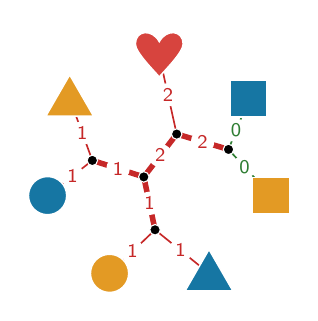
\begin{tikzpicture}[x=1.0cm,y=1.0cm,baseline=(current bounding box.center)]
\coordinate (v1) at (1.13770,0.90728);
\coordinate (v2) at (0.63137,-1.31106);
\coordinate (v3) at (-1.41868,-0.32381);
\coordinate (v4) at (1.41868,-0.32381);
\coordinate (v5) at (-1.13770,0.90728);
\coordinate (v6) at (-0.63137,-1.31106);
\coordinate (v7) at (0.00000,1.45517);
\coordinate (v8) at (0.87924,0.26266);
\coordinate (v9) at (0.22128,0.45821);
\coordinate (v10) at (-0.05387,-0.75780);
\coordinate (v11) at (-0.85011,0.12332);
\coordinate (v12) at (-0.19653,-0.08639);
\draw[g2tree internal,draw=g2Barren] (v8)--(v9);
\draw[g2tree internal,draw=g2Barren] (v9)--(v12);
\draw[g2tree internal,draw=g2Barren] (v10)--(v12);
\draw[g2tree internal,draw=g2Barren] (v11)--(v12);
\draw[g2tree pendant,draw=g2Prime] (v1)--(v8);
\draw[g2tree pendant,draw=g2Barren] (v2)--(v10);
\draw[g2tree pendant,draw=g2Barren] (v3)--(v11);
\draw[g2tree pendant,draw=g2Prime] (v4)--(v8);
\draw[g2tree pendant,draw=g2Barren] (v5)--(v11);
\draw[g2tree pendant,draw=g2Barren] (v6)--(v10);
\draw[g2tree pendant,draw=g2Barren] (v7)--(v9);
\node[g2tree weight,text=g2Barren,font={\sffamily\fontsize{7.5}{8}\selectfont}] at (0.55026,0.36043) {2};
\node[g2tree weight,text=g2Barren,font={\sffamily\fontsize{7.5}{8}\selectfont}] at (0.01237,0.18591) {2};
\node[g2tree weight,text=g2Barren,font={\sffamily\fontsize{7.5}{8}\selectfont}] at (-0.12520,-0.42209) {1};
\node[g2tree weight,text=g2Barren,font={\sffamily\fontsize{7.5}{8}\selectfont}] at (-0.52332,0.01846) {1};
\node[g2tree weight,text=g2Prime,font={\sffamily\fontsize{7.5}{8}\selectfont}] at (0.97616,0.50439) {0};
\node[g2tree weight,text=g2Barren,font={\sffamily\fontsize{7.5}{8}\selectfont}] at (0.27062,-1.01979) {1};
\node[g2tree weight,text=g2Barren,font={\sffamily\fontsize{7.5}{8}\selectfont}] at (-1.10197,-0.07474) {1};
\node[g2tree weight,text=g2Prime,font={\sffamily\fontsize{7.5}{8}\selectfont}] at (1.08153,0.04274) {0};
\node[g2tree weight,text=g2Barren,font={\sffamily\fontsize{7.5}{8}\selectfont}] at (-0.97801,0.47198) {1};
\node[g2tree weight,text=g2Barren,font={\sffamily\fontsize{7.5}{8}\selectfont}] at (-0.34043,-1.03233) {1};
\node[g2tree weight,text=g2Barren,font={\sffamily\fontsize{7.5}{8}\selectfont}] at (0.11064,0.95669) {2};
\node[g2tree vertex] at (v8) {};
\node[g2tree vertex] at (v9) {};
\node[g2tree vertex] at (v10) {};
\node[g2tree vertex] at (v11) {};
\node[g2tree vertex] at (v12) {};
\node[g2tree dark,rectangle,minimum size=4.657500000000001mm,font={\sffamily\fontsize{9}{9}\selectfont\bfseries}] at (v1) {};
\begin{scope}[shift={(v2)},scale=1.0125000000000002,transform shape]
\path[fill=g2TaxonBlue,draw=white,line width=.55pt,line join=round] (0mm,3.0mm)--(-3.0mm,-2.2mm)--(3.0mm,-2.2mm)--cycle;
\end{scope}
\node[g2tree dark,circle,minimum size=4.86mm,font={\sffamily\fontsize{9}{9}\selectfont\bfseries}] at (v3) {};
\node[g2tree light,rectangle,minimum size=4.657500000000001mm,font={\sffamily\fontsize{9}{9}\selectfont\bfseries}] at (v4) {};
\begin{scope}[shift={(v5)},scale=1.0125000000000002,transform shape]
\path[fill=g2TaxonYellow,draw=white,line width=.55pt,line join=round] (0mm,3.0mm)--(-3.0mm,-2.2mm)--(3.0mm,-2.2mm)--cycle;
\end{scope}
\node[g2tree light,circle,minimum size=4.86mm,font={\sffamily\fontsize{9}{9}\selectfont\bfseries}] at (v6) {};
\begin{scope}[shift={(v7)},scale=1.0125000000000002,transform shape]
\path[fill=g2HeartRed,draw=white,line width=.55pt]
  (0mm,-2.7mm)..controls(-.45mm,-2.1mm)and(-3.0mm,.35mm)..(-3.0mm,1.45mm)
  ..controls(-3.0mm,3.2mm)and(-.9mm,3.4mm)..(0mm,1.75mm)
  ..controls(.9mm,3.4mm)and(3.0mm,3.2mm)..(3.0mm,1.45mm)
  ..controls(3.0mm,.35mm)and(.45mm,-2.1mm)..(0mm,-2.7mm)--cycle;
\end{scope}
\end{tikzpicture}
\endgroup
\par}
\vskip 0pt plus 1filll
\noindent\rlap{char\ 2}\par
\end{minipage}
\\
\end{tabular}
\endgroup
\endgroup
